\documentclass{article}
\usepackage[margin=2cm]{geometry}




\usepackage{float}

% Use adjustwidth environment to exceed column width (see example table in text)
\usepackage{changepage}

% Use Unicode characters when possible
\usepackage[utf8]{inputenc}

% textcomp package and marvosym package for additional characters
\usepackage{textcomp,marvosym}

% fixltx2e package for \textsubscript
\usepackage{fixltx2e}

% amsmath and amssymb packages, useful for mathematical formulas and symbols
\usepackage{amsmath,amssymb,amsthm}

% cite package, to clean up citations in the main text. Do not remove.
\usepackage{cite}

% Use nameref to cite supporting information files (see Supporting Information section for more info)
\usepackage{nameref,hyperref}


% ligatures disabled
\usepackage{microtype}
\DisableLigatures[f]{encoding = *, family = * }

% rotating package for sideways tables
\usepackage{rotating}



% Bold the 'Figure #' in the caption and separate it from the title/caption with a period
% Captions will be left justified
\usepackage[aboveskip=1pt,labelfont=bf,labelsep=period,justification=raggedright,singlelinecheck=off]{caption}


% Remove brackets from numbering in List of References
\makeatletter
%\renewcommand{\@biblabel}[1]{\quad#1.}
\makeatother




%% Include all macros below

\newcommand{\lorem}{{\bf LOREM}}
\newcommand{\ipsum}{{\bf IPSUM}}

%% END MACROS SECTION


%%%% Additional user-defined macros

%% Math

% Operators
\DeclareMathOperator{\Cov}{Cov}
\DeclareMathOperator{\Var}{Var}
\DeclareMathOperator{\E}{\mathbb{E}}
\DeclareMathOperator{\Proba}{\mathbb{P}}
\newcommand{\Covb}[2]{\ensuremath{\Cov\!\left[#1,#2\right]}}
\newcommand{\Eb}[1]{\ensuremath{\E\!\left[#1\right]}}
\newcommand{\Pb}[1]{\ensuremath{\Proba\!\left[#1\right]}}
\newcommand{\Varb}[1]{\ensuremath{\Var\!\left[#1\right]}}
\newcommand{\norm}[1]{\| #1 \|}
\newcommand{\indep}{\rotatebox[origin=c]{90}{$\models$}}



\usepackage{ragged2e}


\title{Second-order Control of Complex Systems with Correlated Synthetic Data}
\date{}

\author{Juste Raimbault\textsuperscript{1,2,3,*}\medskip\\
\textsuperscript{1}CASA, UCL, London, UK\\
\textsuperscript{2}UPS CNRS 3611 ISC-PIF, Paris, France\\
\textsuperscript{3}UMR CNRS 8504 G{\'e}ographie-cit{\'e}s, Paris, France\medskip\\
Email : juste.raimbault@polytechnique.edu}

\begin{document}

\maketitle


\begin{abstract} % abstract
\justify
Generation of hybrid synthetic data resembling real data to some criteria is an important methodological and thematic issue in most disciplines which study complex systems. Interdependencies between constituting elements, materialized within respective relations, lead to the emergence of macroscopic patterns. Being able to control the dependance structure and level within a synthetic dataset is thus a source of knowledge on system mechanisms. We describe in this paper a methodology consisting in the generation of synthetic datasets on which correlation structure is controlled. The method is applied in a first example on financial time-series and allows to understand the role of interferences between components at different scales on performances of a predictive model. A second application on a geographical system is then proposed, in which the weak coupling between a population density model and a network morphogenesis model allows to simulate territorial configurations. The calibration on morphological objective on European data and intensive model exploration unveils a large spectrum of feasible correlations between morphological and network measures. We demonstrate therein the flexibility of our method and the variety of possible applications.
\end{abstract}




\justify


%%%%%%%%%%%%%%%%%
\section*{Introduction}



The use of synthetic data, in the sense of statistical populations generated randomly under constraints of proximity of patterns to a studied system, is a widely used methodology, and more particularly in disciplines related to complex systems such as therapeutic evaluation~\cite{abadie2010synthetic}, territorial science~\cite{moeckel2003creating,pritchard2009advances}, machine learning~\cite{bolon2013review} or bio-informatics~\cite{van2006syntren}. It can consist in data disaggregation by creation of a microscopic population with fixed macroscopic properties, or in the creation of new populations at the same scale than a given sample, with criteria of proximity to the real sample. The creation of synthetic populations for microsimulation models is a typical example where empirical statistical distributions are reproduced \cite{muller2010population}. In data extensive contexts, several methods have been developed and improved for a better reproduction of margin distributions \cite{barthelemy2013synthetic}.

The criteria to evaluate the quality of a synthetic dataset will depend on expected applications and can for example vary from a restrictive statistical fit on given indicators, to weaker assumptions of similarity in aggregated patterns. In the case of systems where emergence plays a strong role, a microscopic property does not directly imply given macroscopic patterns, which reproduction is indeed one aim of modeling and simulation practices in complexity science. With the rise of new computational paradigms~\cite{arthur2015complexity}, data (simulated, measured or hybrid) shape our understanding of complex systems. Methodological tools for data-mining and modeling and simulation (including the generation of synthetic data) are therefore crucial to be developed.

% Christian A. W. Bruhn, Stephen Hetterich, Cynthia Schuck-Paim, Esra Kürüm, Robert J. Taylor, Roger Lustig, Eugene D. Shapiro, Joshua L. Warren, Lone Simonsen, and Daniel M. Weinberger, Estimating the population-level impact of vaccines using synthetic controls. : Synthetic Controls


Whereas first order (in the sense of distribution moments) is generally well used, it is not systematic nor simple to control generated data structure at second order, i.e. covariance structure between generated variables. Some specific examples can be found, such as in~\cite{ye2011investigation} where the sensitivity of discrete choices models to the distributions of inputs and to their dependance structure is examined. It is also possible to interpret complex networks generative models~\cite{newman2003structure} as the production of an interdependence structure for a system, contained within link topology. Most methods yielding a high level of accuracy on synthetic covariance structure depend on sampling or data reconstruction methods, and need therefore large datasets. We introduce here a generic method taking into account dependance structure for the generation of synthetic datasets, more precisely with the mean of controlled correlation matrices. It can be applied to cases where microscopic data on the studied system is not available and system similarity is targeted on aggregated indicators. Our contribution relies in this generic methodology, and its application to two very different kind of complex systems.


The rest of the paper is organized as follows. The generic method is formally described, to be then applied on two very different examples, namely financial time-series and territorial spatial configurations. Each example can be read independently and illustrates potentialities of the method and possible technical limitations. We discuss then possible further developments and applications, in particular for the geographical system.


\section*{Method Formalization}


Domain-specific methods aforementioned are too broad to be summarized into a same formalism. We propose therefore here a rather generic and model-agnostic framework, focused on the control of correlations structures in synthetic data.

Let $\vec{X}_I$ a multidimensional stochastic process (that can be indexed e.g. with time in the case of time-series, but also space, or discrete set abstract indexation). We assume given a real dataset $\mathbf{X}=(X_{i,j})$, interpreted as a set of realizations of the stochastic process. We propose to generate a statistical population $\mathbf{\tilde{X}}=\tilde{X}_{i,j}$ such that
\begin{enumerate}
\item a given criteria of proximity to data is verified, i.e. given a precision $\varepsilon$ and an indicator $f$, we have $\norm{f(\mathbf{X})-f(\mathbf{\tilde{X}})} < \varepsilon$
\item level of correlation is controlled, i.e. given a matrix $R$ fixing correlation structure (symmetric matrix with coefficients in $[-1,1]$ and unity diagonal), we have $\hat{\Var{}}\left[(\tilde{X}_i)\right] = \Sigma R \Sigma$, where the standard deviation diagonal matrix $\Sigma$ is estimated on the synthetic population.
\end{enumerate}


The second requirement will generally be conditional to parameter values determining generation procedure, either generation models being simple or complex ($R$ itself is a parameter). Formally, synthetic processes are parametric families $\tilde{X}_i[\vec{\alpha}]$.

We propose to apply the methodology on very different examples, both typical of complex systems: financial high-frequency time-series and territorial systems. We illustrate the flexibility of the method, and claim to help building interdisciplinary bridges by methodology transposition and reasoning analogy. In the first case, proximity to data is the equality of signals at a fundamental frequency, to which higher frequency synthetic components with controlled correlations are superposed. It follows a logic of hybrid data for which hypothesis or model testing is done on a more realistic context than on purely synthetic data. In the second case, morphological calibration of a population density distribution model allows to respect real data proximity. Correlations of urban form with transportation network measures are empirically obtained by exploration of coupling with a network morphogenesis model. The control is in this case indirect as feasible space is empirically determined.

%  : explicit the fact that real data may come out of different parameter values ?


\section*{Correlated financial time-series}


\subsection*{Context}

Our first field of application are financial complex systems, of which captured signals, financial time-series, are heterogeneous, multi-scalar and highly non-stationary~\cite{mantegna2000introduction}. Correlations have already been the object of a broad part of related literature. For example, Random Matrix Theory allows to distinguish signal from noise, or at least to estimate the proportion of information undistinguishable from noise, for a correlation matrix computed for a large number of asset with low-frequency signals (daily returns mostly)~\cite{2009arXiv0910.1205B}. Similarly, Complex Network Analysis on networks constructed from correlations, by methods such as Minimal Spanning Tree~\cite{2001PhyA..299...16B} or more refined extensions developed for this purpose~\cite{tumminello2005tool}, yielded promising results such as the reconstruction of economic sectors structure. At high frequency, the precise estimation of interdependence parameters in the framed of fixed assumptions on asset dynamics, has been extensively studied from a theoretical point of view aimed at refinement of models and estimators~\cite{barndorff2011multivariate}. Theoretical results must be tested on synthetic datasets as they ensure a control of most parameters in order to check that a predicted effect is indeed observable all things being otherwise equal. Empirical confirmation of estimator improvement is obtained on a synthetic dataset at a fixed correlation level.


We consider a network of assets $(X_i(t))_{1\leq i \leq N}$ sampled at high-frequency (typically 1s). We use a multi-scalar framework (used e.g. in wavelet analysis approaches~\cite{ramsey2002wavelets} or in multi-fractal signal processing~\cite{bouchaud2000apparent}) to interpret observed signals as the superposition of components at different time scales : $X_i=\sum_{\omega}{X_i^{\omega}}$. We denote by $T_i^{\omega} = \sum_{\omega' \leq \omega} X_i^{\omega}$ the filtered signal at a given frequency $\omega$. A recurrent problem in the study of complex systems is the prediction of a trend at a given scale. It can be viewed as the identification of regularities and their distinction from components considered as random. For the sake of simplicity, we represent such a process as a trend prediction model at a given temporal scale $\omega_1$, formally an estimator $M_{\omega_1} : (T_i^{\omega_1}(t'))_{t'<t} \mapsto \hat{T_i}^{\omega_1}(t)$ which aims to minimize error on the real trend $\norm{T_i^{\omega_1} - \hat{T}_i^{\omega_1}}$. In the case of autoregressive multivariate estimators, the performance will depend among other parameters on respective correlations between assets. It is thus interesting to apply the method to the evaluation of performance as a function of correlation at different scales. We assume a Black-Scholes dynamic for assets~\cite{jarrow1999honor}, i.e. $dX = \sigma\cdot dW$, with $W$ Wiener process. Such a dynamic model allows an easy modulation of correlation levels.


      
%%%%%%%%%%%%%%%%%%%
\begin{figure}[h!]
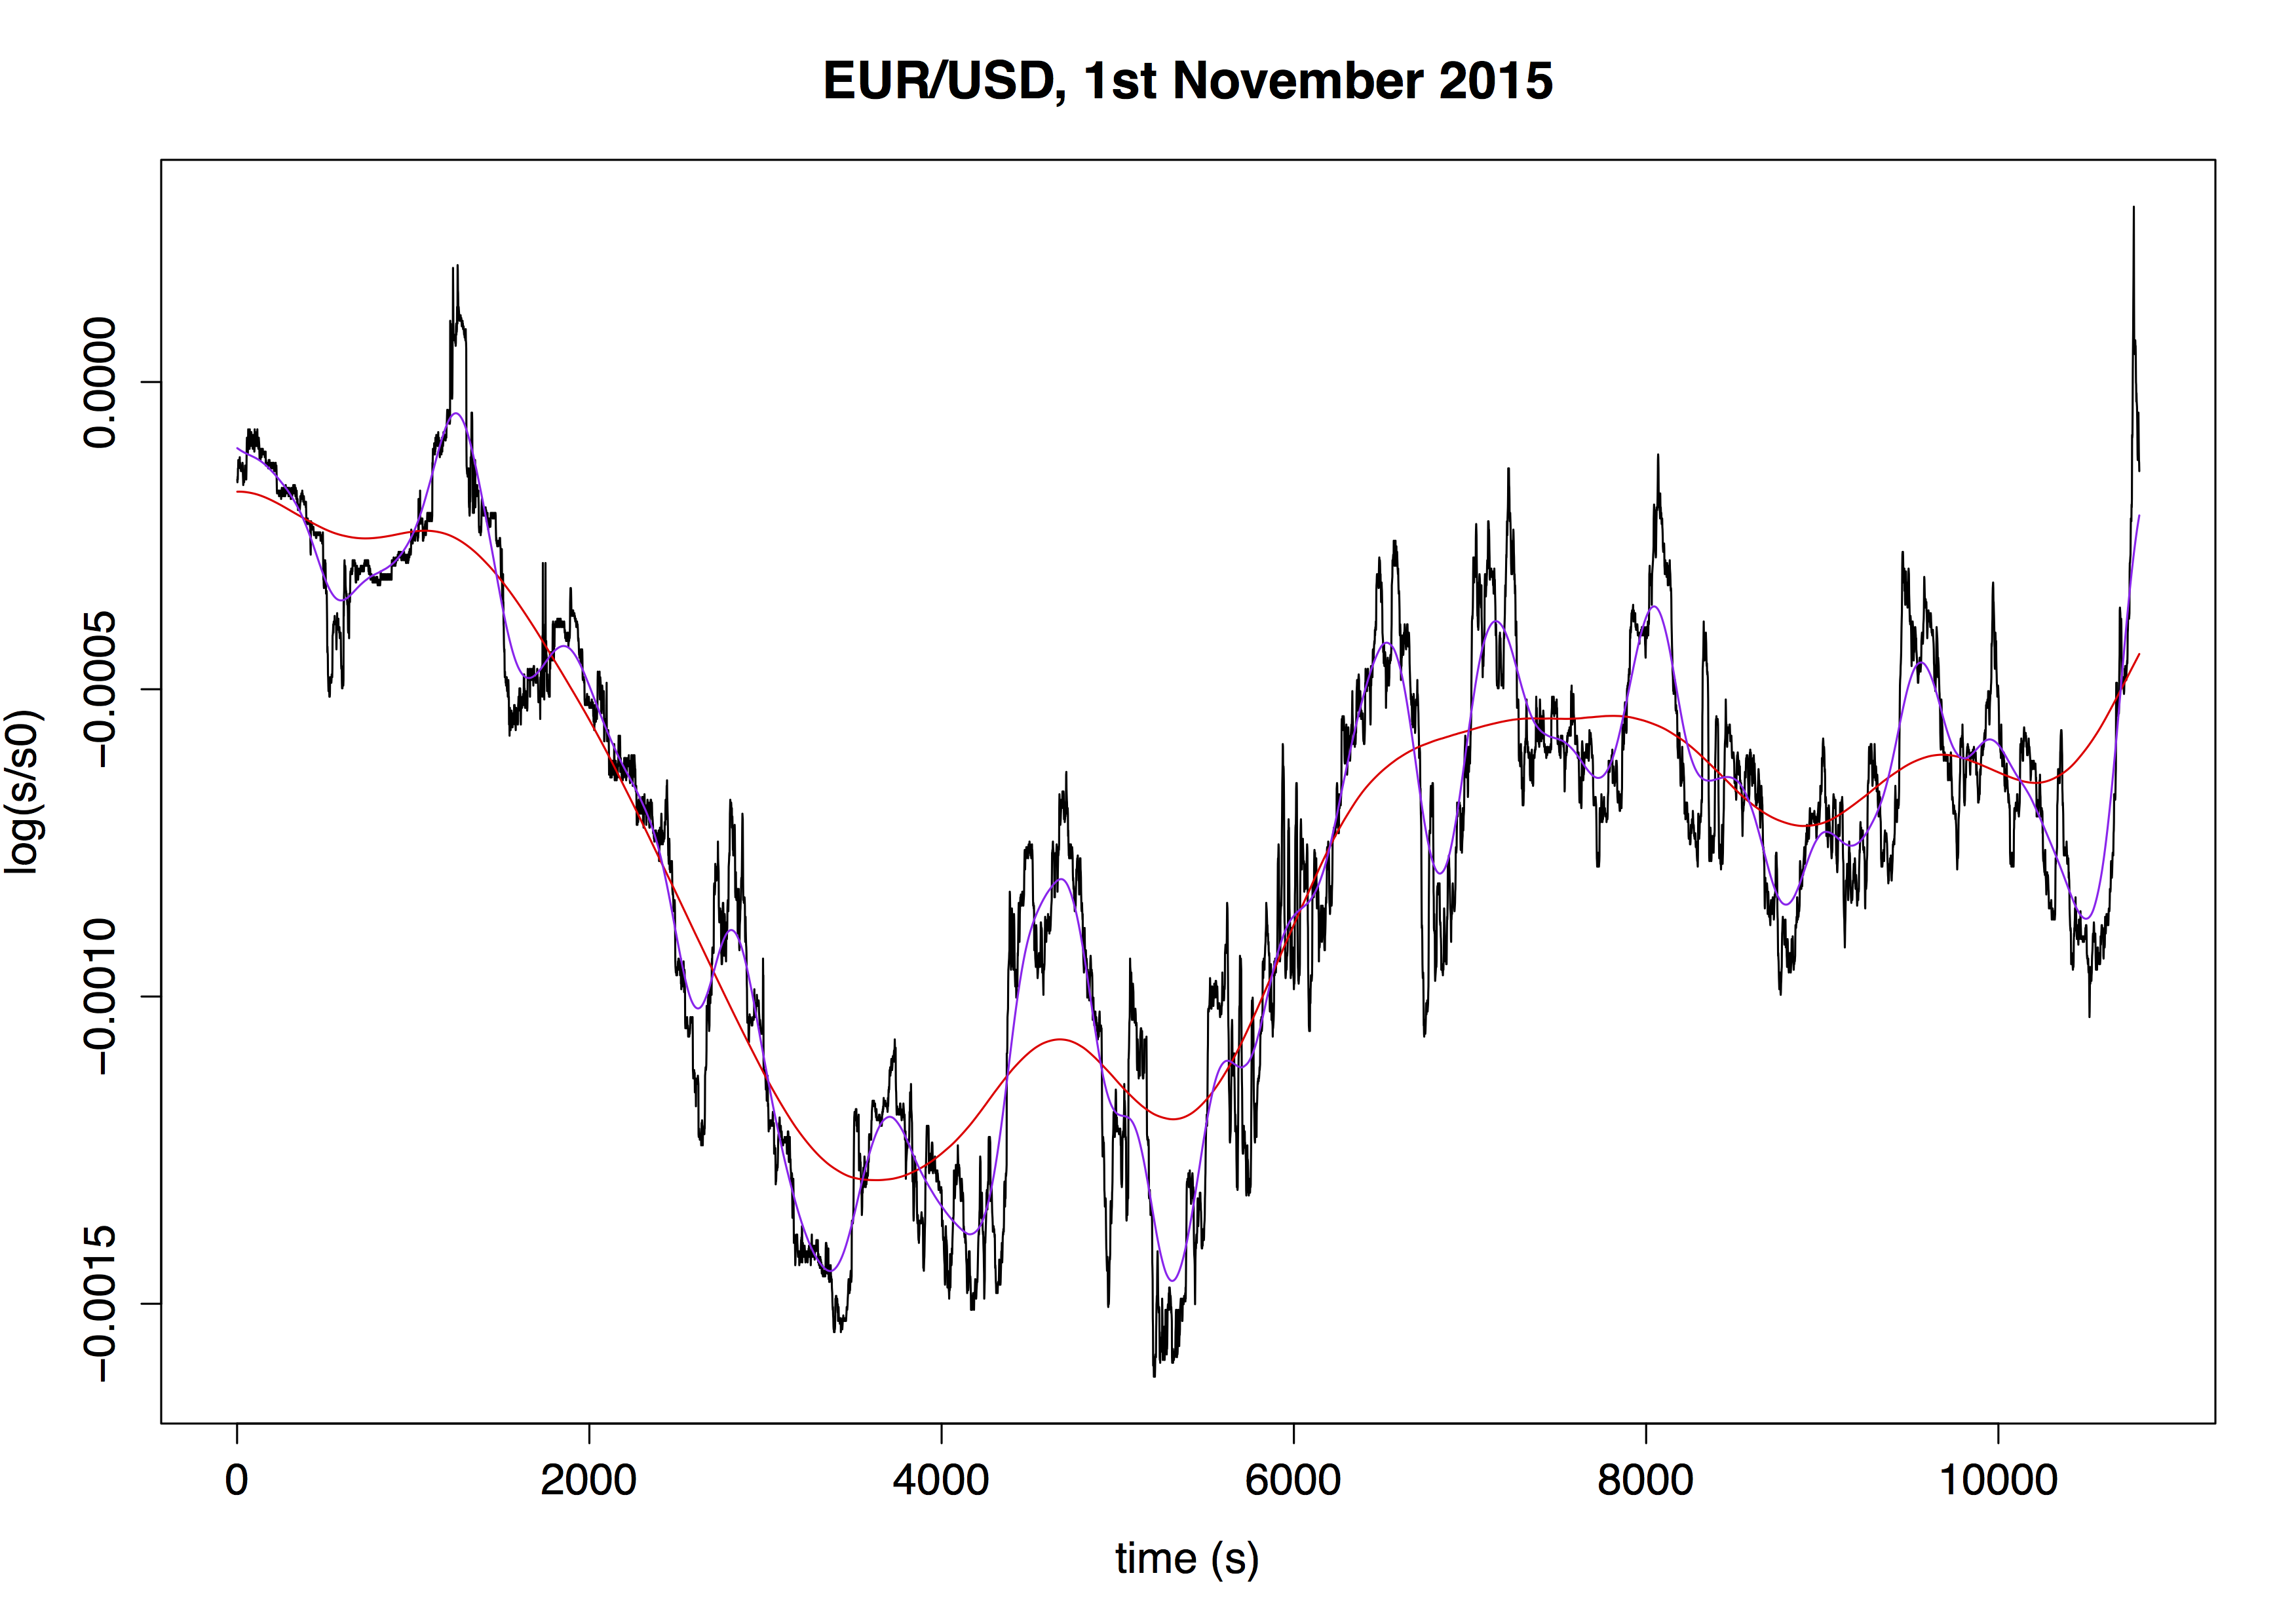
\includegraphics[width=\columnwidth]{ex_filtering.png}
\caption{\textbf{Example of the multi-scalar structure of the signal, basis of the construction of synthetic signals.} \emph{Log-prices} are represented on a time window of around 3h for November 1st 2015 for asset EUR/USD, with 10min (purple) and 30min trends.\label{fig:example_signal}}
\end{figure}
%%%%%%%%%%%%%%%%%%%

\subsection*{Data generation}


We can straightforward generate $\tilde{X}_i$ such that $\Varb{\tilde{X}_i^{\omega_1}}=\Sigma R \Sigma$ (with $\Sigma$ estimated standard deviations and $R$ fixed correlation matrix) and verifying $X_i^{\omega \leq \omega_0} = \tilde{X}_i^{\omega \leq \omega_0}$. This means in practice that the data proximity indicator is the identity of components at a lower frequency than a fundamental frequency $\omega_0 < \omega_1$. We use therefore the simulation of Wiener processes with fixed correlation. Indeed, if $dW_1 \indep dW_1^{\indep}$ (and $\sigma_1 < \sigma_2$ indicatively, assets being interchangeable), then
\[
W_2 = \rho_{12}W_1 + \sqrt{1-\frac{\sigma_1^2}{\sigma_2^2}\cdot\rho_{12}^2}\cdot W_1^{\indep}
\]
is such that $\rho(dW_1,dW_2)=\rho_{12}$. Signals for other components can be constructed the same way by Gram orthonormalization. We isolate the component at the desired frequency $\omega_1$ by filtering the signal, i.e. $\tilde{X}_i^{\omega_1} = W_i - \mathcal{F}_{\omega_0}[W_i]$ (with $\mathcal{F}_{\omega_0}$ low-pass filter with cut-off frequency $\omega_0$). We reconstruct then the hybrid synthetic signals by taking
 
\begin{equation}
\tilde{X}_i = T_i^{\omega_0} + \tilde{X}_i^{\omega_1}
\end{equation}



\subsection*{Methodology}

The method is tested on an example with two assets from foreign exchange market (EUR/USD and EUR/GBP), on a six month period from June 2015 to November 2015. Data was obtained from \url{http://www.histdata.com/}. The data cleaning procedure, starting from original series sampled at a frequency around 1s, consists in a first step to the determination of the minimal common temporal range (missing sequences being ignored, by vertical translation of series, i.e. $S(t):=S(t)\cdot \frac{S(t_{n})}{S(t_{n-1})}$ when $t_{n-1},t_n$ are extremities of the ``hole'' and $S(t)$ value of the asset, what is equivalent to keep the constraint to have returns at similar temporal steps between assets). We study then \emph{log-prices} and \emph{log-returns} \cite{mantegna1999introduction}, defined by $X(t):=\log{\frac{S(t)}{S_0}}$ and $\Delta X (t) = X(t) - X(t-1)$. Raw data are filtered at a maximal frequency $\omega_m = 10\textrm{min}$ (which will be the maximal frequency for following treatments) for concerns of computational efficiency. As time-series are then sampled at $3\cdot\omega_m$ to avoid aliasing, a day of size 86400 for 1s sampling is reduced to a much smaller size of 432. We use a non-causal gaussian filter of total width $\omega$. We fix the fundamental frequency $\omega_0=24\textrm{h}$ and we propose to construct synthetic data at frequencies $\omega_1 = 30\textrm{min},1\textrm{h},2\textrm{h}$. See Fig.~\ref{fig:example_signal} for an example of signal structure at these different scales.

% For the respect of copyright, only cleaned and filtered at $\omega_m$ data are made openly available.




It is crucial to consider the interference between $\omega_0$ and $\omega_1$ frequencies in the reconstructed signal: the correlation which is indeed estimated is 
\[
\rho_{e} = \rho \left[ \Delta \tilde{X}_1 , \Delta \tilde{X}_2 \right] = \rho \left[ \Delta T_1^{\omega_0} + \Delta \tilde{X}_1^{\omega} , \Delta T_2^{\omega_0} + \Delta \tilde{X}_2^{\omega}\right]
\]


Assuming to be in the reasonable limit $\sigma_1 \gg \sigma_0$ (fundamental frequency small enough), that $\Covb{\Delta \tilde{X}_i^{\omega_1}}{\Delta X_j^{\omega}}=0$ for all $i,j,\omega_1 > \omega$ and that returns are centered at any scale, we can develop the previous expression to compute the correction on effective correlation due to interferences. We obtain at the first order the expression of effective correlation given by


\begin{equation}
\label{eq:eff_corr}
\rho_e = \left[ \varepsilon_1 \varepsilon_2 \rho_0 + \rho \right] \cdot \left[ 1 - \frac{1}{2}\left(\varepsilon_1^2 + \varepsilon_2^2 \right) \right]
\end{equation}

{\noindent}what corresponds to the correlation that we can effectively simulate in synthetic data.

Correlation is in practice estimated with a Pearson estimator, the covariances being corrected for bias, i.e.
\[
\hat{\rho}[X1,X2] = \frac{\hat{C}[X1,X2]}{\sqrt{\hat{\Var{}}[X1] \cdot \hat{\Var{}}[X2]}}
\]

, where $\hat{C}[X1,X2] = \frac{1}{(T-1)}\sum_{t} X_1(t)X_2(t) - \frac{1}{T\cdot (T-1)} \sum_t X_1(t) \sum_t X_2(t)$ and $\hat{\Var{}}[X] = \frac{1}{T}\sum_t{X^2(t)}-\left(\frac{1}{T}\sum_tX(t)\right)^2$.


The generated synthetic data are then used to test a toy model. We propose in particular to investigate the predictive power of a very simple linear model. The tested predictive model $M_{\omega_1}$ is a simple \emph{ARMA} for which parameters $p=2,q=0$ are fixed (as we do not create lagged correlation, we do not expect large orders of auto-regression as these kind of processes have short memory for real data; furthermore smoothing is not necessary as data are already filtered). It is however applied in an adaptive way, in the sense that given a time window $T_W$, we estimate for any $t$ the model on $[t-T_W+1,t]$ in order to predict signals at $t+1$.

%  the adaptation level staying rather low, as parameters $T_W,p,q$ and model type do not vary
% We are positioned within the framework of~\cite{potiron2016estimating} which assumes a locally parametric dynamic but for which meta-parameters are fixed. We could imagine a variable $T_W$ which would adapt for the best local fit, the same way parameters are estimated in bayesian signal processing by augmentation of the state with parameters.}.


%\paragraph{Implementation}

Experiments are implemented in the \texttt{R} language, using in particular the \texttt{MTS}~\cite{Tsay:2015xy} library for time-series models. Cleaned data and source code are available on an open \texttt{git} repository at \url{https://github.com/JusteRaimbault/SynthAsset}.



%%%%%%%%%%%%%%%%%%%
\begin{figure}[h!]
\centering
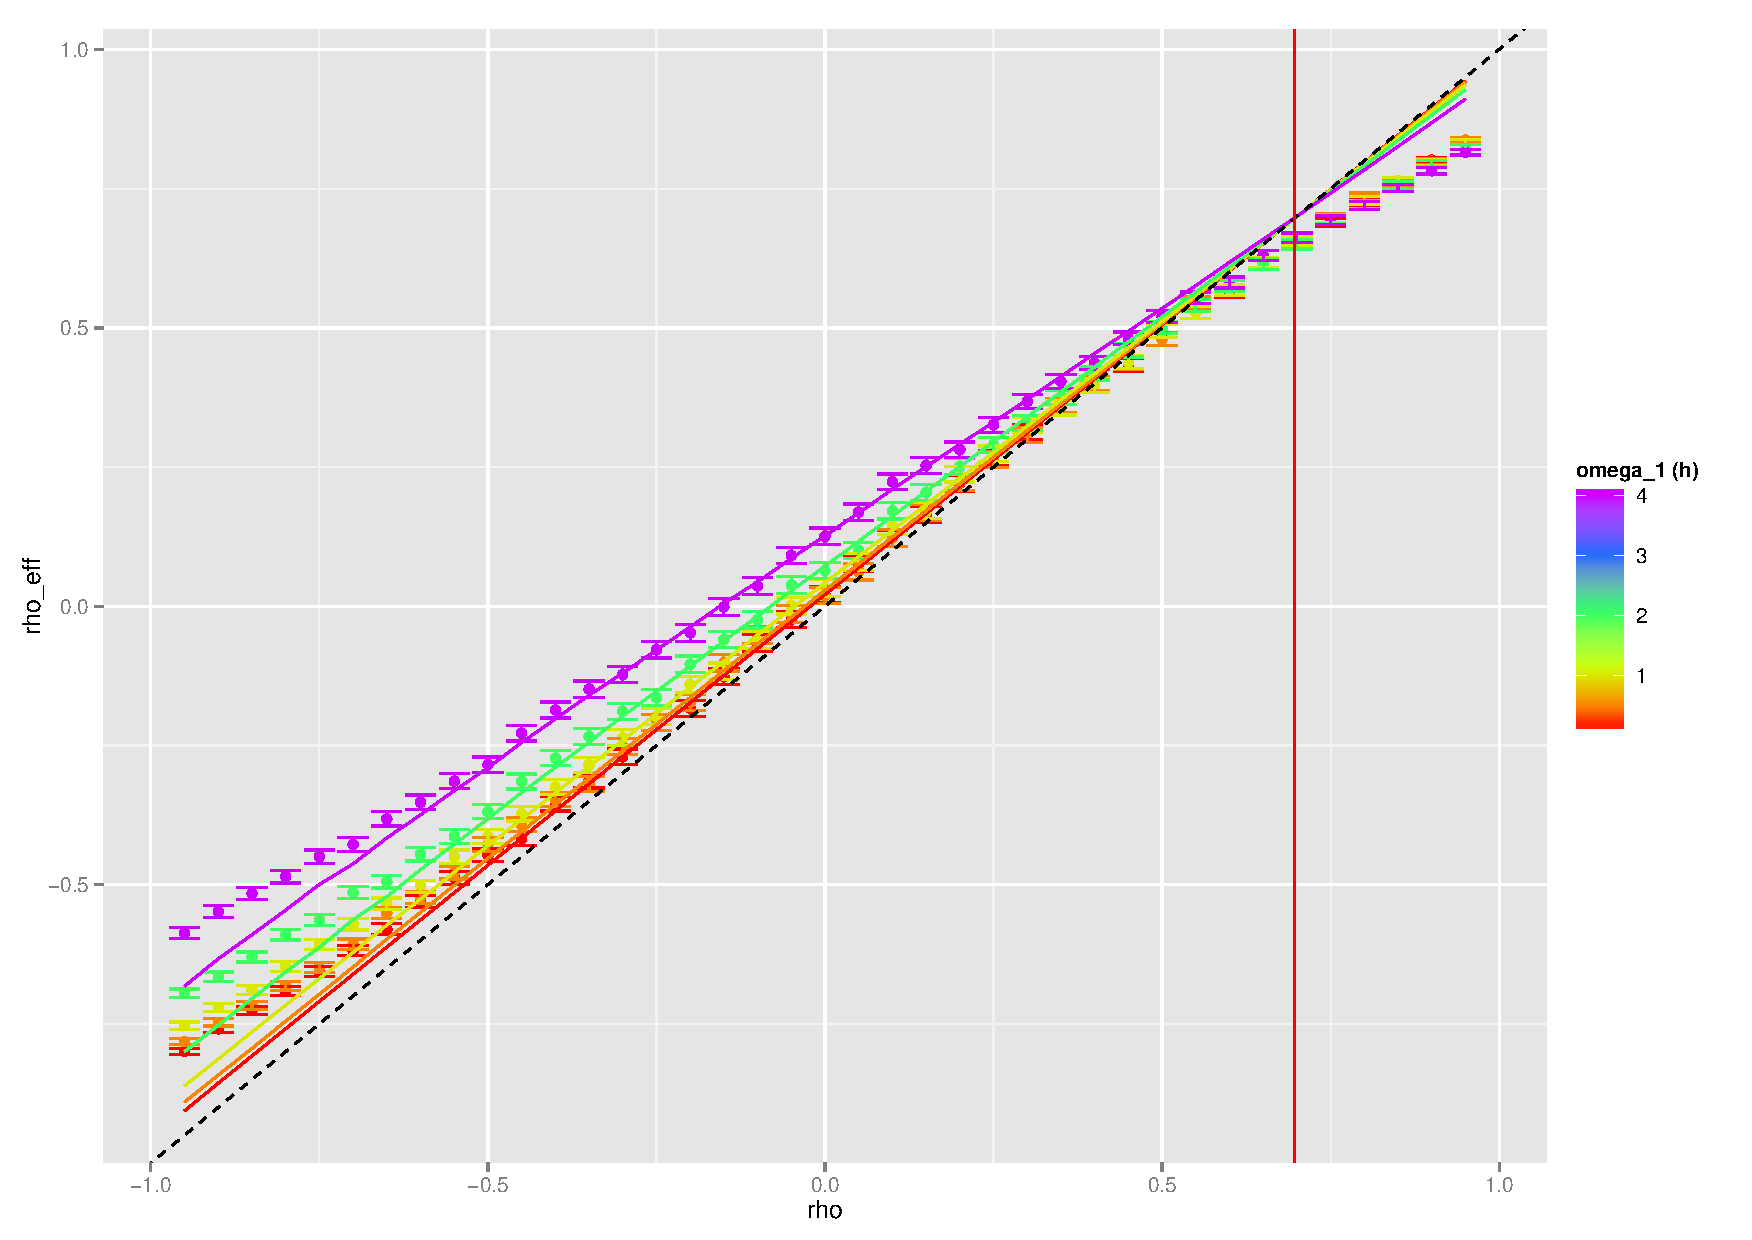
\includegraphics[width=\columnwidth]{effectiveCorrs_withGoodTh_A4}
\caption{\textbf{Effective correlations obtained on synthetic data.} Dots represent estimated correlations on a synthetic dataset corresponding to 6 months between June and November 2015 (error-bars give 95\% confidence intervals obtained with standard Fisher method) ; scale color gives filtering frequency $\omega_1=10\textrm{min},30\textrm{min},1\textrm{h},2\textrm{h},4\textrm{h}$ ; solid lines give theoretical values for $\rho_e$ obtained by~\ref{eq:eff_corr} with estimated volatilities (dotted-line diagonal for reference) ; vertical red line position is the theoretical value such that $\rho = \rho_e$ with mean values for $\varepsilon_i$ on all points. We observe for high absolute correlations values a deviation from corrected values, what should be caused by non-verified independence and centered returns assumptions. Asymmetry is caused by the high value of $\rho_0 \simeq 0.71$.}
\label{fig:effective_corrs}
\end{figure}
%%%%%%%%%%%%%%%%%%%


%%%%%%%%%%%%%%%%%%%
\begin{figure}[h!]
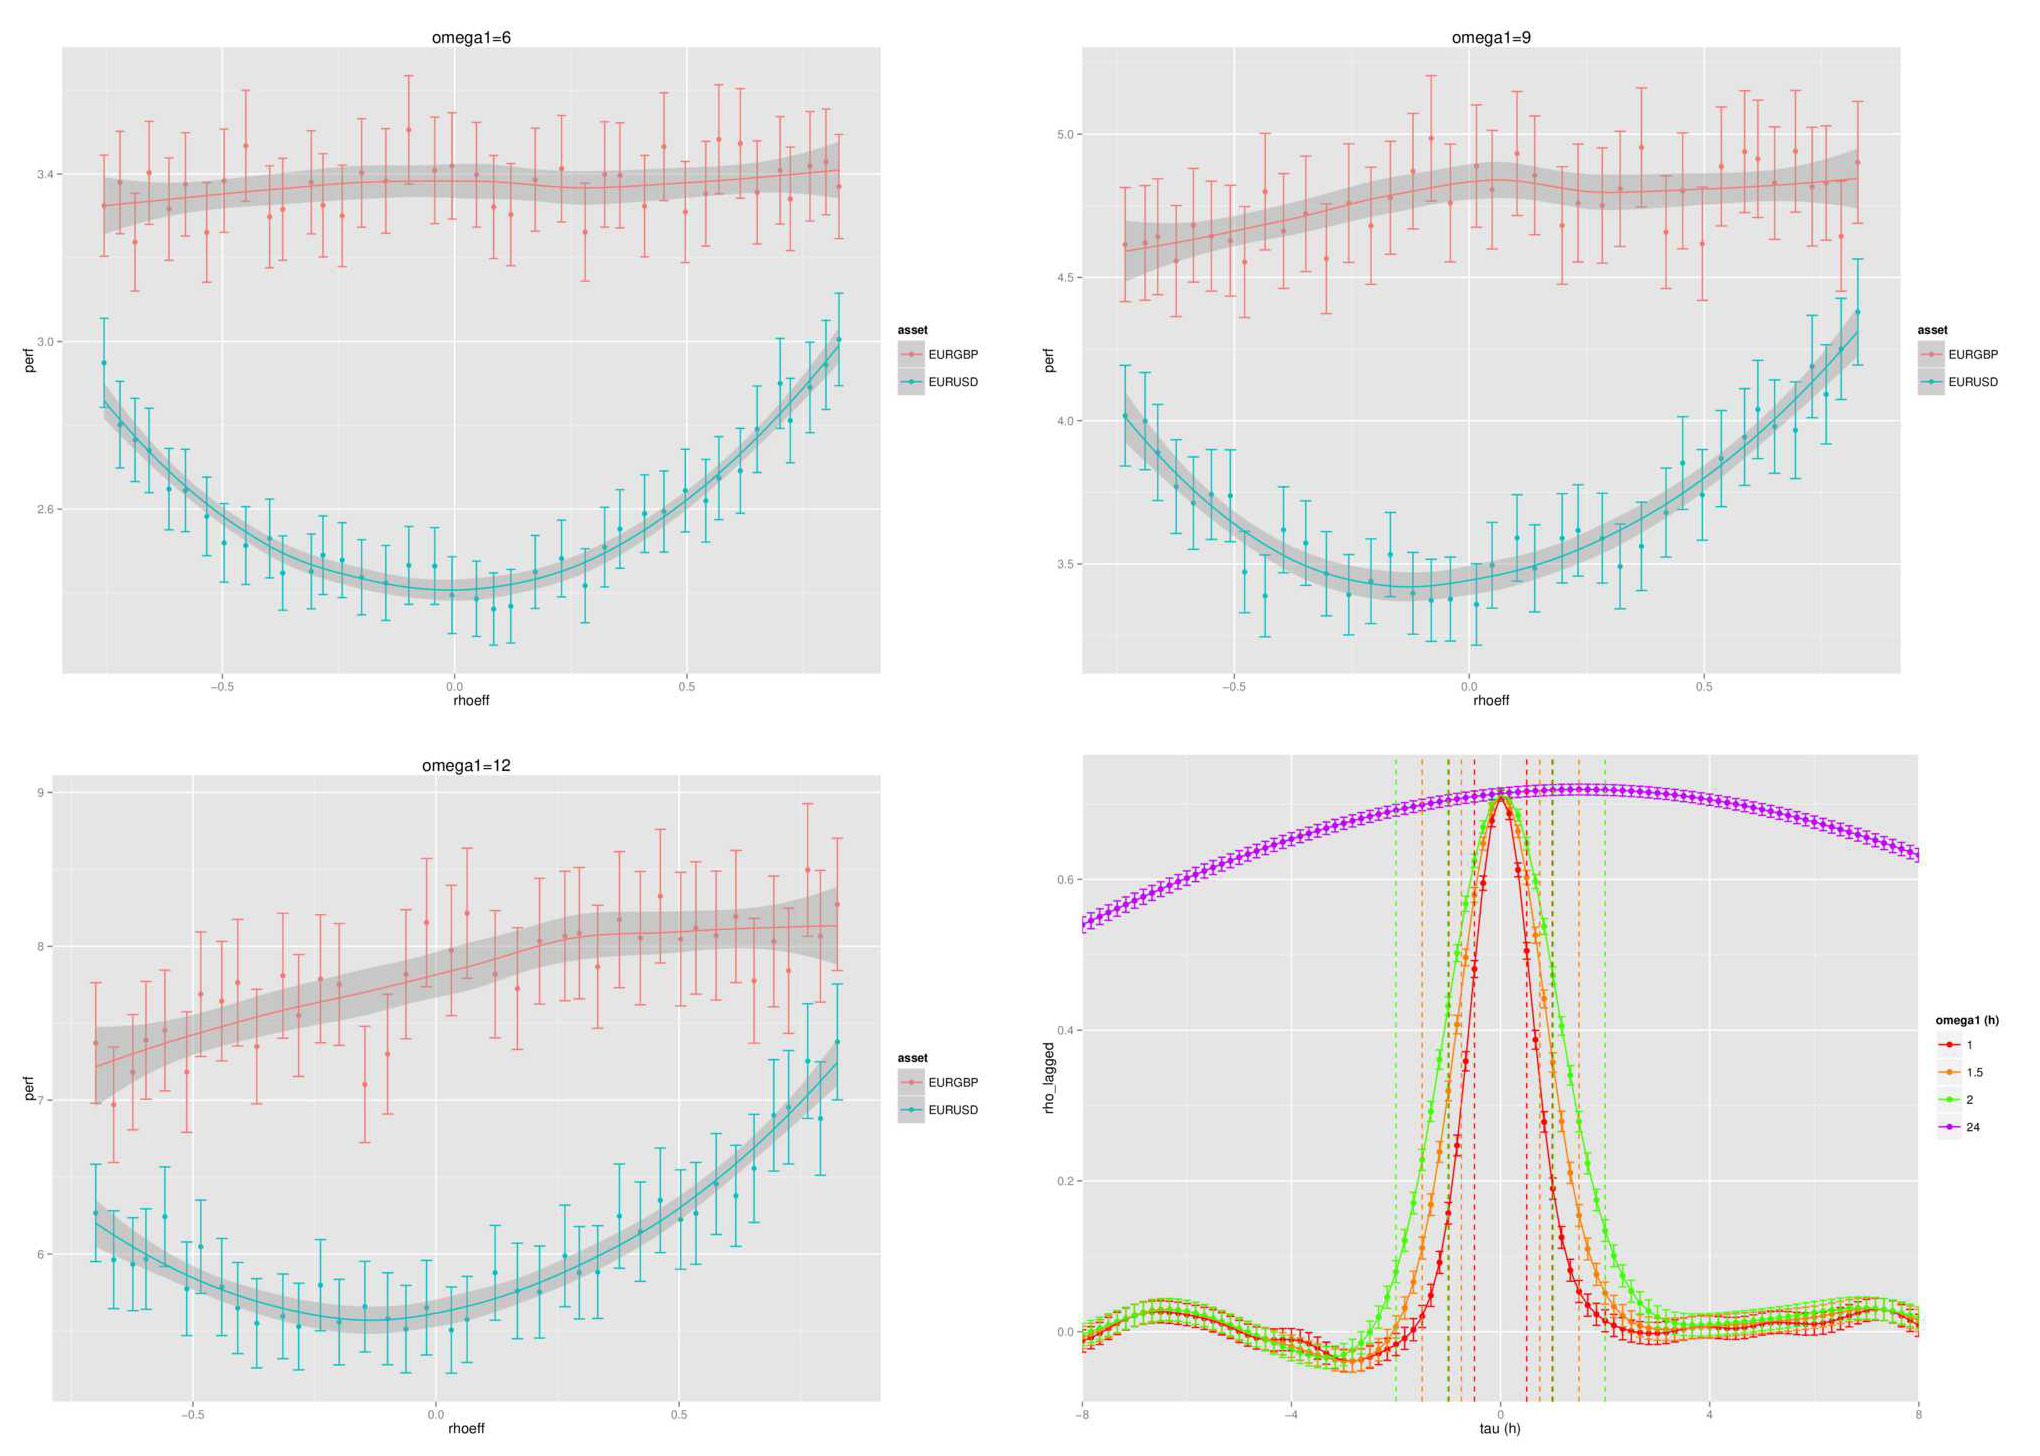
\includegraphics[width=\linewidth]{C-syntheticdata-model_perf.jpg}
\caption{\textbf{Performance of a predictive model as a function of simulated correlations.} From left to right and top to bottom, three first graphs show for each asset the normalized performance of an ARMA model ($p=2,q=0$), defined as $\pi = \left(\frac{1}{T}\sum_t\left(\tilde{X}_i(t) - M_{\omega_1}\left[\tilde{X}_i\right](t)\right)^2 \right) / \sigma \left[ \tilde{X}_i \right]^2$ (95\% confidence intervals computed by $\pi = \bar{\pi} \pm (1.96\cdot \sigma [\pi])/\sqrt{T}$, local polynomial smoothing to ease reading). It is interesting to note the U-shape for EUR/USD, due to interference between components at different scales. Correlation between simulated noises deteriorates predictive power. The study of lagged correlations (here $\rho [\Delta X_{\textrm{EURUSD}}(t),\Delta X_{\textrm{EURGBP}}(t-\tau)]$) on real data clarifies this phenomenon: the fourth graph show an asymmetry in curves at any scale compared to zero lag $(\tau = 0)$ what leads fundamental components to increase predictive power for the dollar, amelioration then perturbed by correlations between simulated components. Dashed lines show time steps (in equivalent $\tau$ units) used by the ARMA at each scale, what allows to read the corresponding lagged correlation on fundamental component.\label{fig:model_perf}}
\end{figure}
%%%%%%%%%%%%%%%%%%%



\subsection*{Results}



Figure~\ref{fig:effective_corrs} shows the effective correlations computed on synthetic data. For standard parameter values (for example $\omega_0=24\textrm{h}$, $\omega_1=2\textrm{h}$ and $\rho=-0.5$), we find $\rho_0\simeq 0.71$ et $\varepsilon_i \simeq 0.3$ what yields $\left| \rho_e - \rho \right|\simeq 0.05$. We observe a good agreement between observed $\rho_e$ and values predicted by~\ref{eq:eff_corr} in the interval $\rho \in [-0.5,0.5]$. On the contrary, for larger absolute values, a deviation increasing with $\left|\rho\right|$ and as $\omega_1$ decreases : it confirms the intuition that when frequency decreases and becomes closer to $\omega_0$, interferences between the two components are not negligible anymore and invalidate independence assumptions for example.



We apply then the predictive model described above to synthetic data, in order to study its mean performance as a function of correlation between signals. Results for $\omega_1 = 1\textrm{h},1\textrm{h}30,2\textrm{h}$ are shown in Fig.~\ref{fig:model_perf}. The a priori counter-intuitive result of a maximal performance at vanishing correlation for one of the assets confirms the role of synthetic data to better understand system mechanisms : the study of lagged correlations shows an asymmetry in the real data that we can understand at a daily scale as an increased influence of EUR/GBP on EUR/USD with a rough two hours lag. The existence of this \emph{lag} allows a ``good'' prediction of EUR/USD thanks to fundamental component. This predictive power is perturbed by added noises in a way that increases with their correlation. The more noises correlated are, the more he model will take them into account and will make false predictions because of the markovian character of simulated brownian (note that the model used has theoretically no predictive power at all on pure brownians).


This case study on a \emph{toy-model} illustrates the relevance of using simulated synthetic data. Further developments can be directed towards the simulation of more realistic data (presence of consistent \emph{lagged correlation} patterns, more realistic models than Black-Scholes) and apply it on more operational predictive models.





%%%%%%%%%%%%%%%%
\section*{Geographical data: correlated population density and road network}

We now turn to a different type of system, namely geographical systems of human settlements, in the particular case here of population distribution in correlation with road network. In this exemple, no theoretical derivation can be done previously to correlated data generation, and simulation appears as a crucial step to implement the method.
 

%%%%%%%%%%%%%%%%%%%%%%
\subsection*{Context}


The use of synthetic data in geography is generally directed towards the generation of synthetic populations within agent-based models (mobility, land-use transport interaction models)~\cite{pritchard2009advances}. We can make a weak link with some techniques in spatial analysis. The extrapolation of a continuous spatial field from a discrete spatial sample through a kernel density estimation for example can be understood as the creation of a synthetic dataset (even if it is not generally the initial view, as in Geographically Weighted Regression~\cite{brunsdon1998geographically} in which variable size kernels do not reconstruct data in a strict sense but extrapolate abstract variables representing interaction between explicit variables). In the field of modeling in quantitative geography, \emph{toy-models} or hybrid models require a consistent initial spatial configuration. A set of possible initial configurations becomes a synthetic dataset on which the model is tested. The first Simpop model~\cite{sanders1997simpop}, precursor of a large family of models later parametrized with real data \cite{pumain2012multi}, could enter that frame but was studied on an unique synthetic spatialization. Similarly underlined was the difficulty to generate an initial transportation infrastructure in the case of the SimpopNet model~\cite{schmitt2014modelisation} although it was admitted as a cornerstone of knowledge on the behavior of the model. A systematic control of spatial configuration effects on the behavior of simulation models was recently proposed~\cite{raimbault2018space}, approach that can be interpreted as a statistical control on spatial data. The aim is to be able to distinguish proper effects due to intrinsic model dynamics from particular effects due to the geographical structure of the case study. Such results are essential for the validation of conclusions obtained with modeling and simulation practices in quantitative geography.




\subsection*{Territorial configuration model}

We propose in our case to generate territorial systems summarized in a simplified way as a spatial population density $d(\vec{x})$ and a transportation network $n(\vec{x})$. Correlations we aim to control are correlations between urban morphological measures and network measures. The question of interactions between territories and networks is already well-studied~\cite{offner1996reseaux} but remains highly complex and difficult to quantify~\cite{offner1993effets}. A dynamical modeling of implied processes should shed light on these interactions \cite{bretagnolle:tel-00459720}. We develop in that frame a simple coupling (i.e. without any feedback loop) between a density distribution model and a network morphogenesis model.




\subsubsection*{Density model}

We use a model $D$ similar to aggregation-diffusion models~\cite{batty2006hierarchy} to generate a discrete spatial distribution of population density. A generalization of the basic model is proposed in~\cite{raimbault2018calibration}, providing a calibration on morphological objectives (entropy, hierarchy, spatial auto-correlation, mean distance) against real values computed on the set of 50km sized grid extracted from European density grid~\cite{eurostat}. We recall here rapidly the processes in the model. An square grid of width $N$, initially empty, is represented by population $(P_i(t))_{1\leq i\leq N^2}$. At each time step, until the total population reaches a fixed parameter $P_m$,
\begin{itemize}
\item total population is increased of a fixed number $N_G$ (growth rate), following a preferential attachment such that $\Pb{P_i(t+1)=P_i(t)+1|P(t+1)=P(t)+1}=\frac{(P_i(t)/P(t))^{\alpha}}{\sum(P_i(t)/P(t))^{\alpha}}$
\item a fraction $\beta$ of population is diffused to four closest neighbors is operated $n_d$ times
\end{itemize}


The two opposite processes of urban concentration and urban sprawl are captured by the model, what allows to reproduce with a good precision a large number of existing morphologies regarding macroscopic urban form indicators.


\subsubsection*{Network model}


On the other hand, we are able to generate a planar transportation network by a model $N$, at a similar scale and given a density distribution. Because of the conditional nature to the density of the generation process, we will first have conditional estimators for network indicators, and secondly natural correlations between network and urban shapes should appear as processes are not independent. The nature and modularity of these correlations as a function of model parameters are still to determine by exploration of the coupled model.



The heuristic network generation procedure is the following :
\begin{enumerate}
\item A fixed number $N_c$ of centers that will be first nodes of the network si distributed given density distribution, following a similar law to the aggregation process, i.e. the probability to be distributed in a given patch is $\frac{(P_i/P)^{\alpha}}{\sum (P_i/P)^{\alpha}}$. Population is then attributed according to Voronoi areas of centers, such that a center cumulates population of patches within its extent.
\item Centers are connected deterministically by percolation between closest clusters : as soon as network is not connected, two closest connected components in the sense of minimal distance between each vertices are connected by the link realizing this distance. It yields a tree-shaped network.
\item Network is modulated by potential breaking in order to be closer from real network shapes. More precisely, a generalized gravity potential between two centers $i$ and $j$ is defined by
\[
V_{ij}(d) = \left[ (1 - k_h) + k_h \cdot \left( \frac{P_i P_j}{P^2} \right)^{\gamma} \right]\cdot \exp{\left( -\frac{d}{r_g (1 + d/d_0)} \right)}
\]
where $d$ can be euclidian distance $d_{ij}=d(i,j)$ or network distance $d_N(i,j)$, $k_h \in [0,1]$ a weight to modulate role of populations, $\gamma$ giving shape of the hierarchy across population values, $r_g$ characteristic interaction distance and $d_0$ distance shape parameter.
\item A fixed number $K\cdot N_L$ of potential new links is taken among couples having greatest euclidian distance potential ($K=5$ is fixed).
\item Among potential links, $N_L$ are effectively realized, that are the one with smallest rate $\tilde{V}_{ij} = V_{ij}(d_N)/V_{ij}(d_{ij})$. At this stage only the gap between euclidian and network distance is taken into account : $\tilde{V}_{ij}$ does indeed not depend on populations and is increasing with $d_N$ at constant $d_{ij}$.
\item Planarity of the network is imposed by creating nodes at possible intersections formed by new links.
\end{enumerate}


We insist on the fact that the network generation procedure is entirely heuristic and result of thematic assumptions (connected initial network, gravity-based link creation) combined with trial-and-error during first explorations. Other model types could be used as well, such as biological self-generated networks~\cite{tero2010rules}, local network growth based on geometrical constraints optimization~\cite{courtat2011mathematics}, or a more complex percolation model than the initial one that would allow the creation of loops for example. We could thus in the frame of a modular architecture, in which the choice between different implementations of a functional brick can be seen as a meta-parameter~\cite{cottineau2015growing}, choose network generation function adapted to a specific need (as e.g. proximity to real data, constraints on output indicators, variety if generated forms, etc. ).



%\paragraph{Parameter space}

Parameter space for the coupled model is constituted by density generation parameters $\vec{\alpha}_D = (P_m/N_G , \alpha,\beta , n_d)$ (we study for the sake of simplicity the rate between population and growth rate instead of both varying, i.e. the number of steps needed to generate the distribution) and network generation parameters $\vec{\alpha}_N=(N_C,k_h,\gamma , r_g , d_0)$. We denote $\vec{\alpha} = (\vec{\alpha}_D,\vec{\alpha}_N)$. 

% \footnote{Weak coupling allows to limit the total number of parameters as a strong coupling would involve retroaction loops and consequently associated parameters to determine their structure and intensity. In order to diminish it, an integrated model would be preferable to a strong coupling, what is slightly different in the sense where it is not possible in the integrated model to freeze one of the subsystems to obtain a model of the other subsystem that would correspond to the non-coupled model.}


%\paragraph{Indicators}

Urban form and network structure are quantified by numerical indicators in order to modulate correlations between these. Morphology is defined as a vector $\vec{M}=(r,\bar{d},\varepsilon,a)$ giving spatial auto-correlation (Moran index), mean distance, entropy and hierarchy (see~\cite{le2015forme} for a precise definition of these indicators). Network measures $\vec{G} = (\bar{c},\bar{l},\bar{s},\delta)$ are with network denoted $(V,E)$
\begin{itemize}
\item Mean centrality $\bar{c}$ defined as average \emph{betweeness-centrality} (normalized in $[0,1]$) on all links.
\item Mean path length $\bar{l}$ given by $\frac{1}{d_m}\frac{2}{|V|\cdot (|V|-1)}\sum_{i<j}d_N(i,j)$ with $d_m$ normalization distance taken here as world diagonal $d_m=\sqrt{2}N$.
\item Mean network speed~\cite{banos2012towards} which corresponds to network performance compared to direct travel, defined as $\bar{s} = \frac{2}{|V|\cdot (|V|-1)}\sum_{i<j}{\frac{d_{ij}}{d_N(i,j)}}$.
\item Network diameter $\delta = \max_{ij}d_N(i,j)$.
\end{itemize}



%\paragraph{Covariance and correlation}

We study the cross-correlation matrix $\Covb{\vec{M}}{\vec{G}}$ between morphology and network. We estimate it on a set of $n$ realizations at fixed parameter values $(\vec{M}\left[D(\vec{\alpha})\right],\vec{G}\left[N(\vec{\alpha})\right])_{1\leq i\leq n}$ with standard unbiased estimator. We estimate correlation with associated Pearson estimator. 




%%%%%%%%%%%%%%%%%%%%%%
\subsection*{Results}


Coupling of generative models is done both at formal and operational levels. We interface therefore independent implementations. The OpenMole software~\cite{reuillon2013openmole} for intensive model exploration offers for that the ideal frame thanks to its modular language allowing to construct \emph{workflows} by task composition and interfacing with diverse experience plans and outputs. For operational reasons, density model is implemented in \texttt{scala} language as an OpenMole plugin, whereas network generation is implemented in agent-oriented language \texttt{NetLogo}~\cite{wilensky1999netlogo} because of its possibilities for interactive exploration and heuristic model construction. Source code is available for reproducibility on an open git repository at \url{https://github.com/JusteRaimbault/CityNetwork/tree/master/Models/Synthetic}.


%%%%%%%%%%%%%%
\begin{figure}[h!]
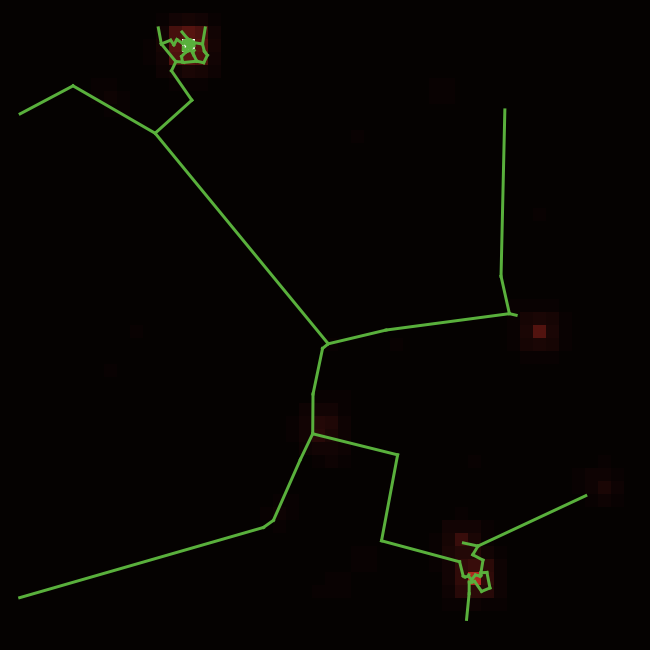
\includegraphics[width=0.45\linewidth]{1_param71861_seed0}
   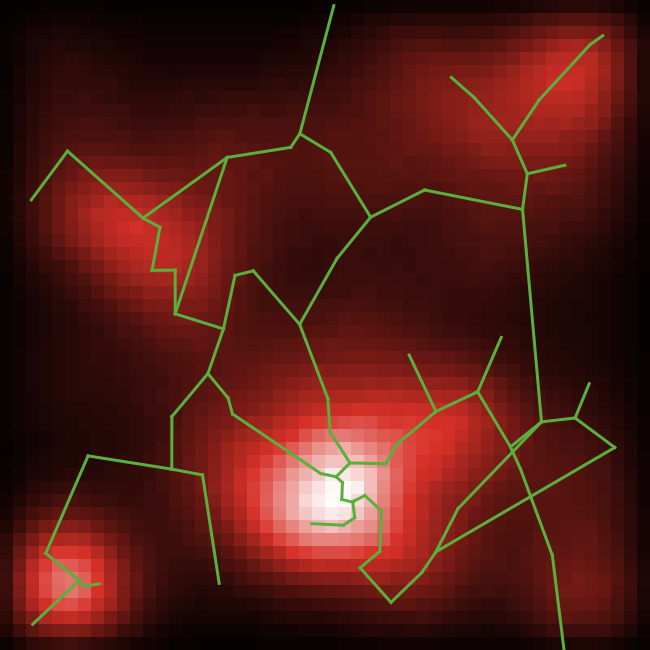
\includegraphics[width=0.45\linewidth]{2_param71913_seed10}\\
   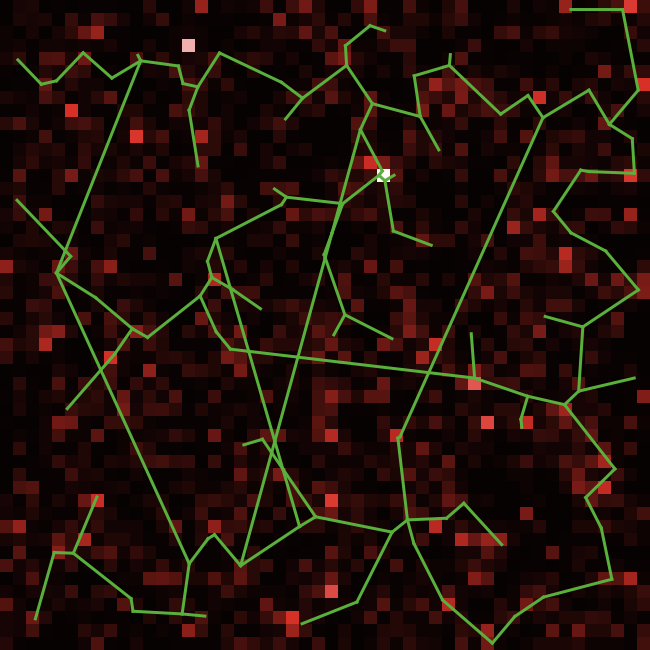
\includegraphics[width=0.45\linewidth]{3_param71918_seed0}
   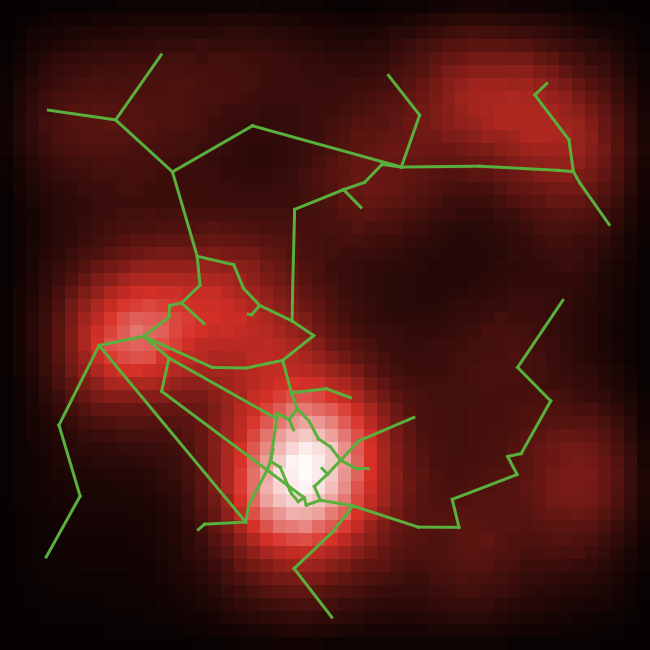
\includegraphics[width=0.45\linewidth]{4_param71945_seed0}
	\caption{\textbf{Configurations obtained for parameters giving the four emphasized points in Fig.~\ref{fig:densnwcor}, in order from left to right and top to bottom.} We recognize polycentric city configurations (2 and 4), diffuse rural settlements (3) and aggregated weak density area (1). See appendice for exhaustive parameter values, indicators and corresponding correlations. For example $\bar{d}$ is highly correlated with $\bar{l},\bar{s}$ ($\simeq$0.8) in (1) but not for (3) although both correspond to rural environments ; in the urban case we observe also a broad variability : $\rho[\bar{d},\bar{c}]\simeq 0.34$ for (4) but $\simeq-0.41$ for (2), what is explained by a stronger role of gravitation hierarchy in (2) $\gamma=3.9,k_h=0.7$ (for (4), $\gamma=1.07,k_h=0.25$), whereas density parameters are similar.\label{fig:configexamples}}
\end{figure}
%%%%%%%%%%%%%%


%%%%%%%%%%%%%%
\begin{figure}[h!]
\begin{minipage}{0.55\linewidth}
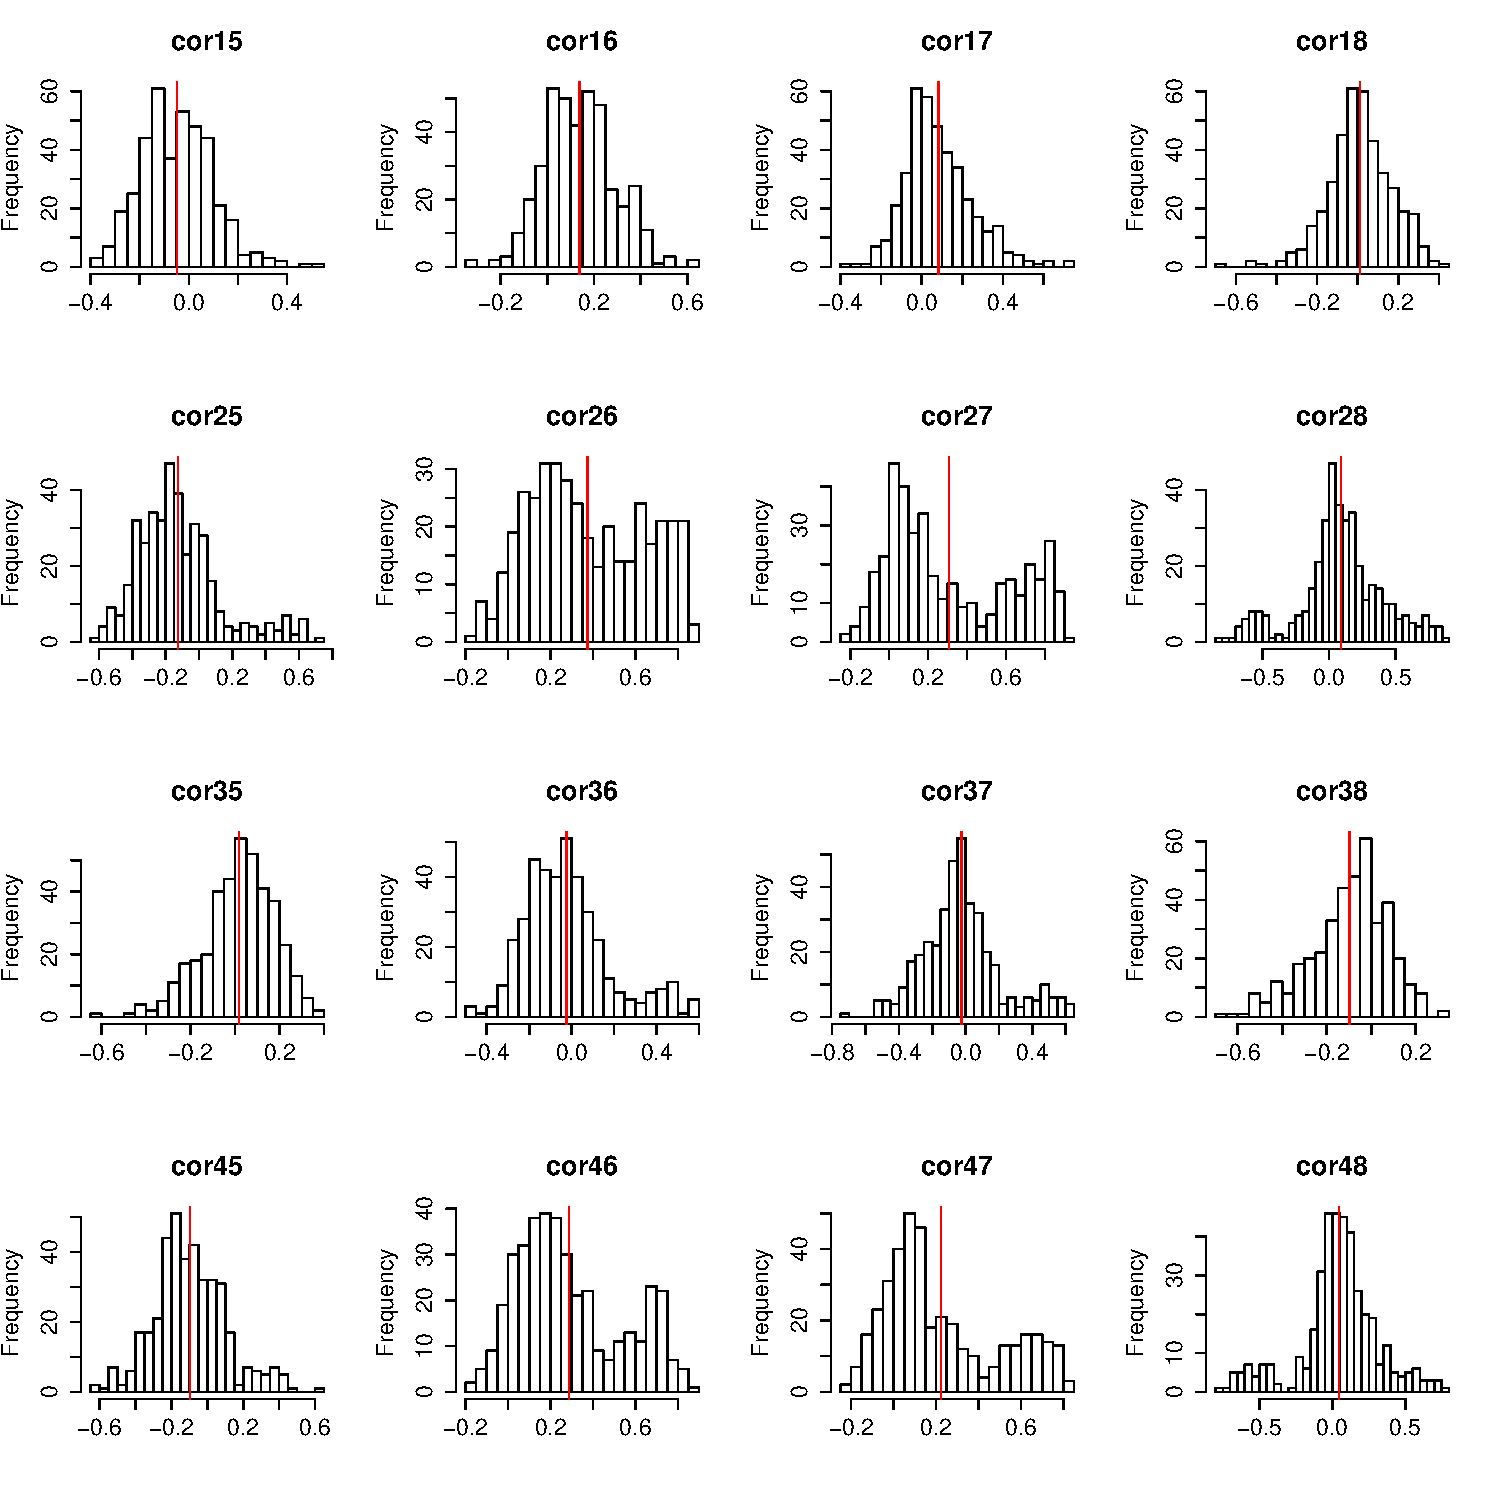
\includegraphics[width=\textwidth]{hist_crossCorMat_breaks30}
\end{minipage}
\begin{minipage}{0.34\linewidth}
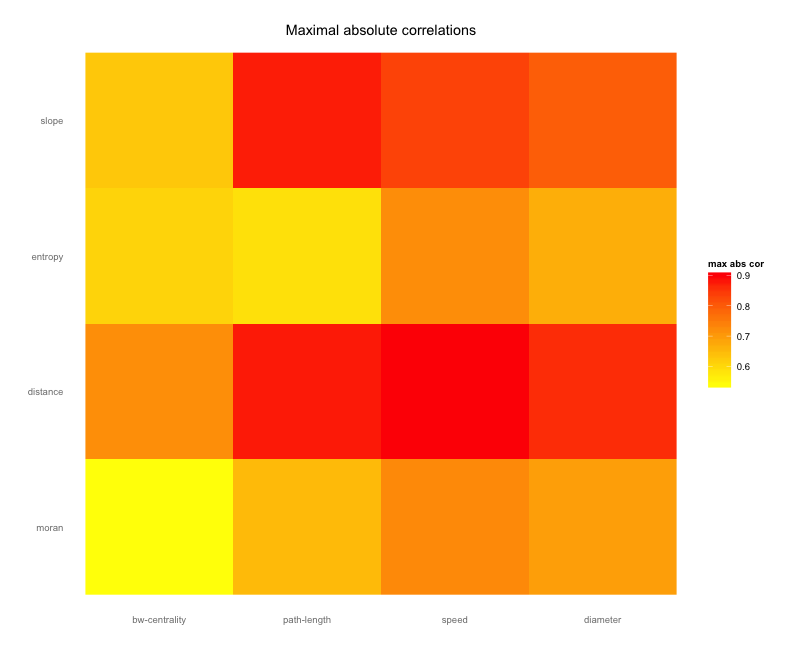
\includegraphics[width=\textwidth]{heatmap_maxAbsCor}\\
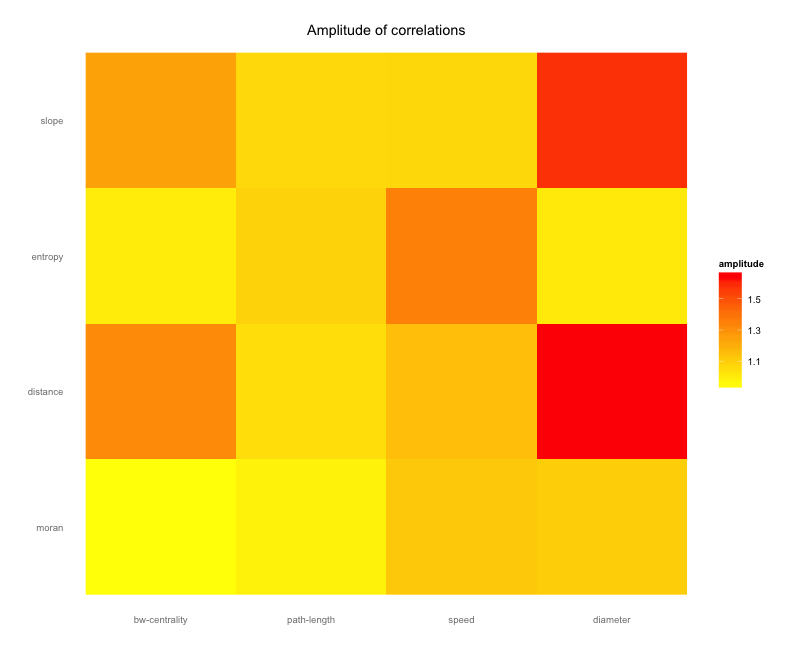
\includegraphics[width=\textwidth]{heatmap_amplCor}
\end{minipage}\\
\begin{minipage}{0.45\linewidth}
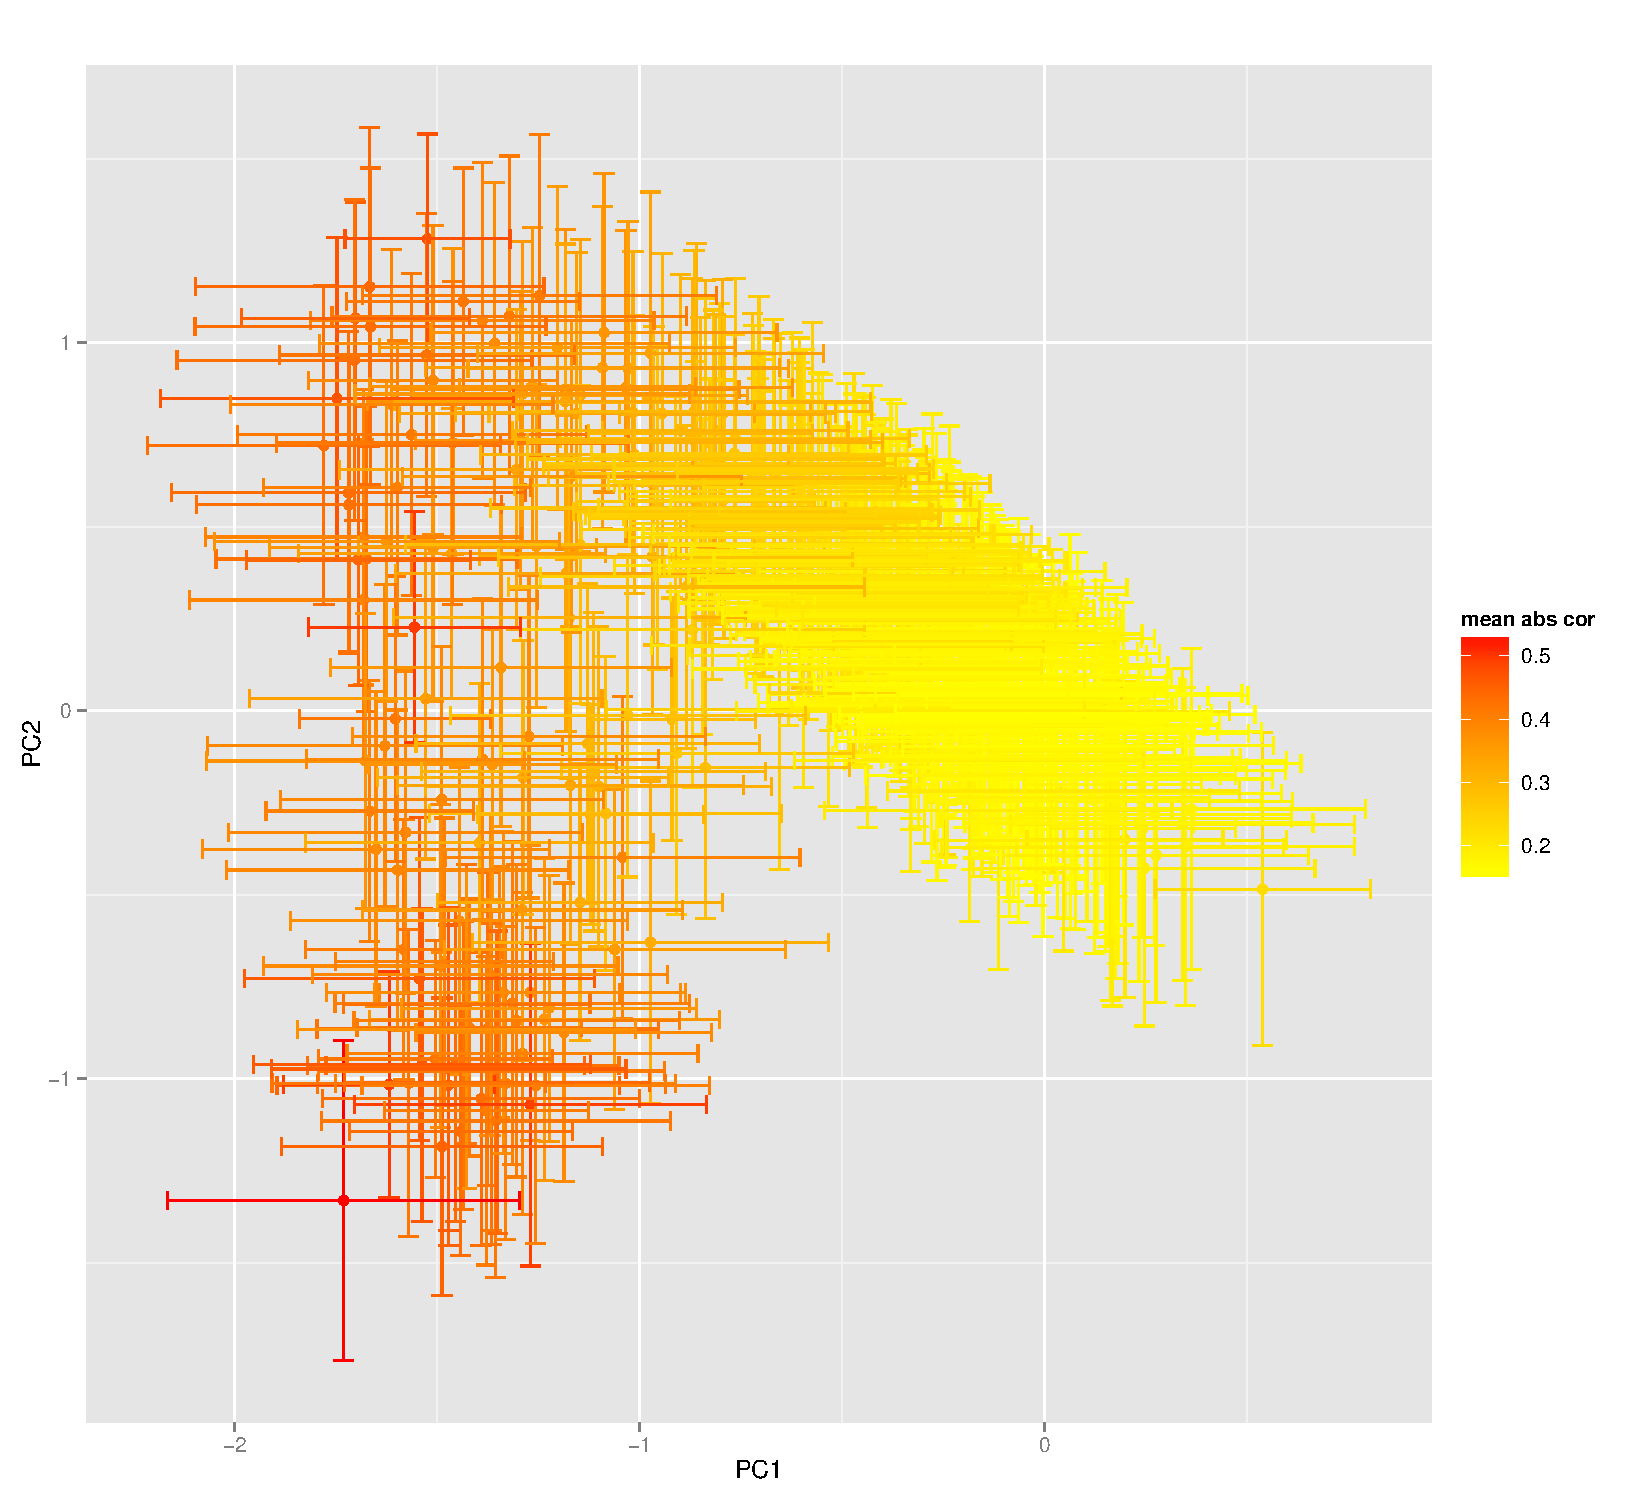
\includegraphics[width=\textwidth]{pca_meanAbsCor_errorBars}
\end{minipage}
\begin{minipage}{0.45\linewidth}
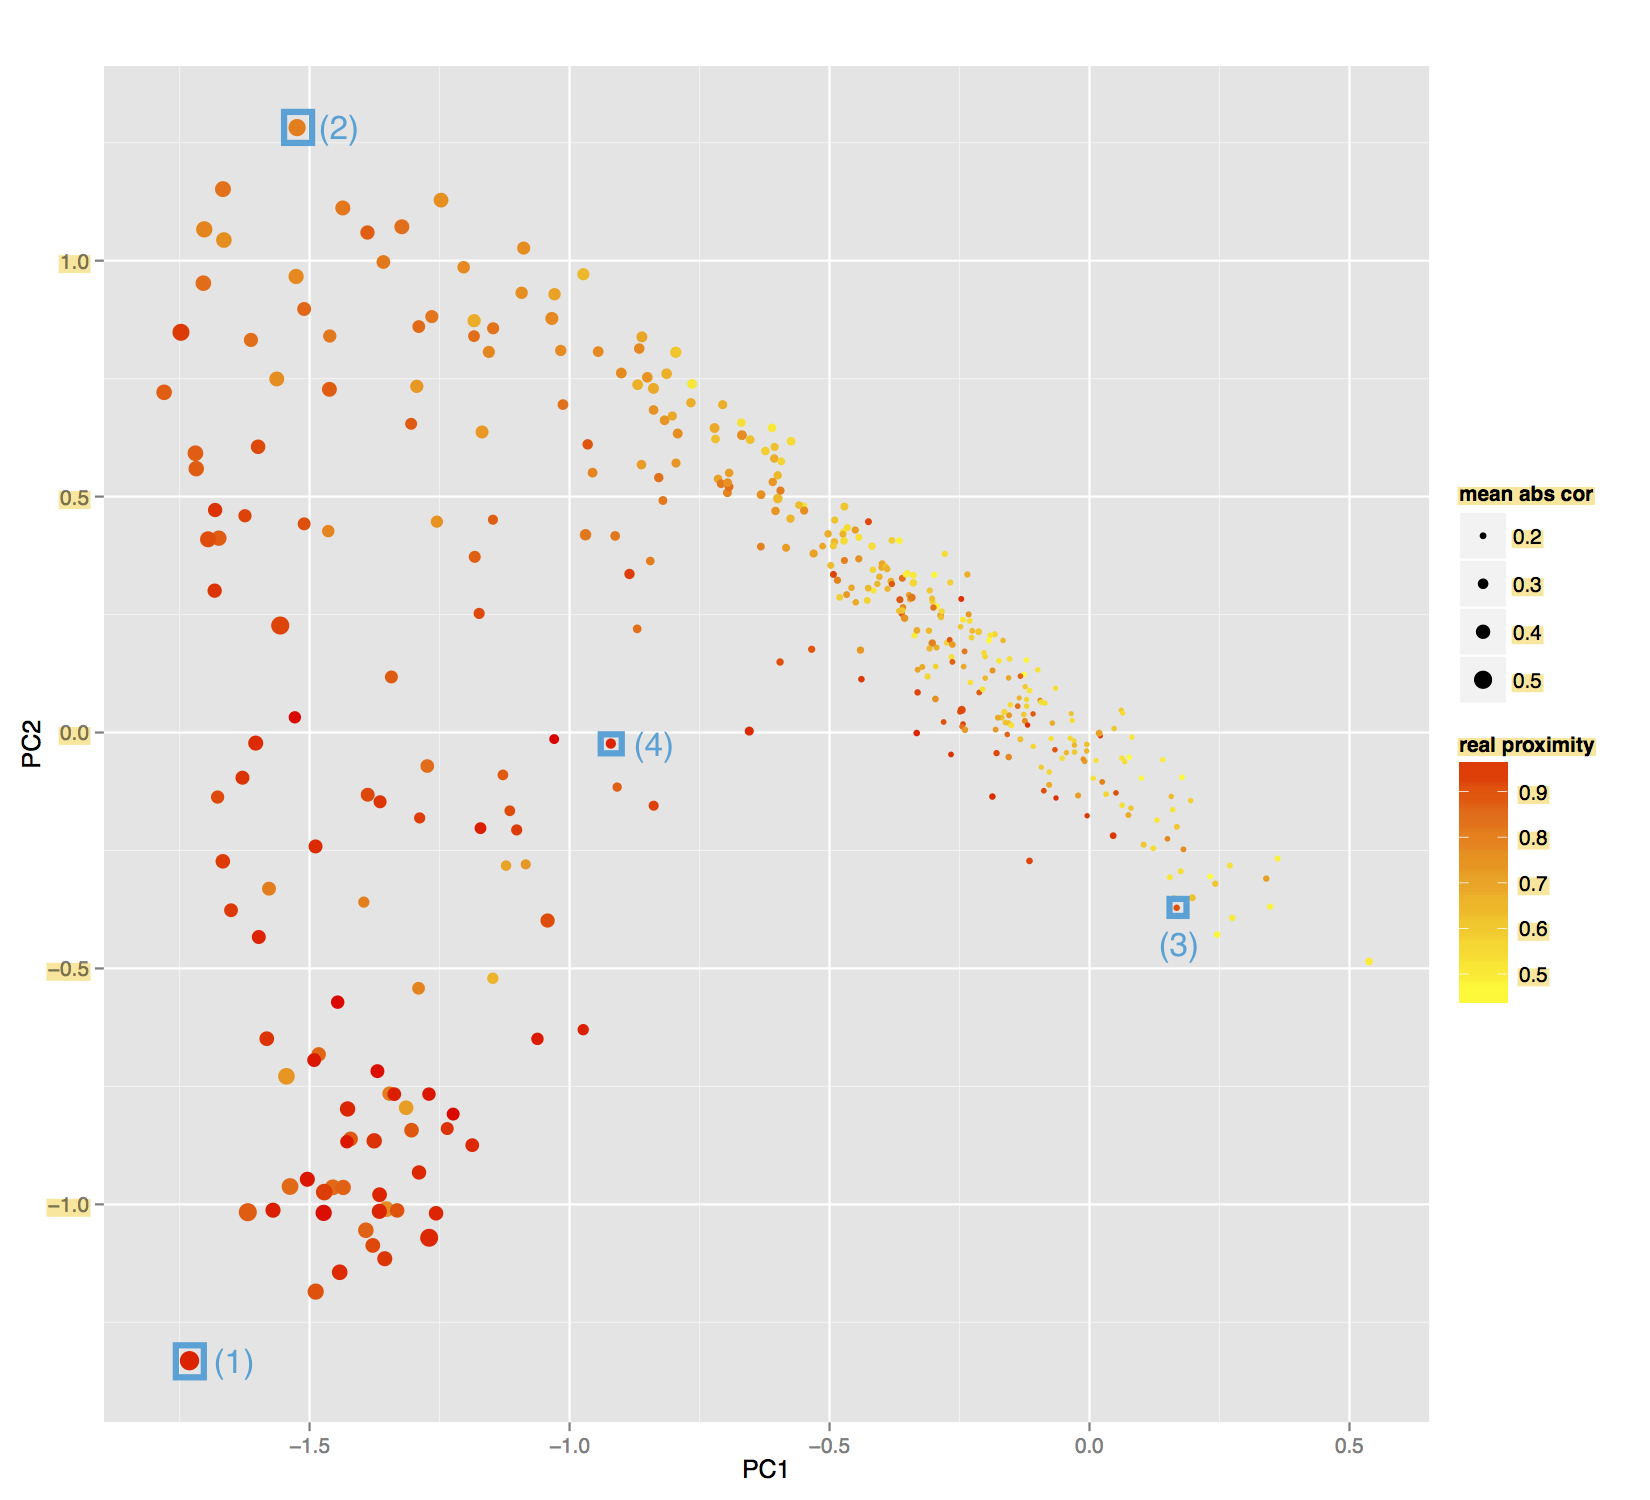
\includegraphics[width=\textwidth]{pca_realDistCol_meanAbsCorSize_withSpecificPoints}
\end{minipage}
\caption{\textbf{Exploration of feasible space for correlations between urban morphology and network structure.} \textbf{(Top left)} Statistical distribution of crossed-correlations between vectors $\vec{M}$ of morphological indicators (in numbering order Moran index, mean distance, entropy, hierarchy) and $\vec{N}$ of network measures (centrality, mean path length, speed, diameter). \textbf{(Top right)} Heatmaps for amplitude of correlations, defined as $a_{ij}=\max_k{\rho_{ij}^{(k)}}-\min_k{\rho_{ij}^{(k)}}$ and maximal absolute correlation, defined as $c_{ij}=\max_k\left| \rho_{ij}^{k} \right|$. \textbf{(Bottom left)} Projection of correlation matrices in a principal plan obtained by Principal Component Analysis on matrix population (cumulated variances: PC1=38\%, PC2=68\%). Error bars are initially computed as 95\% confidence intervals on each matrix element (by standard Fisher asymptotic method), and upper bounds after transformation are taken in principal plan. Scale color gives mean absolute correlation on full matrices. \textbf{(Botton right)} Representation in the principal plan, scale color giving proximity to real data defined as $1 - \min_r \norm{\vec{M}-\vec{M}_r}$ where $\vec{M}_r$ is the set of real morphological measures, point size giving mean absolute correlation. The points highlighted in blue correspond to the configurations shown in Fig.~\ref{fig:configexamples}.\label{fig:densnwcor}}
\end{figure}
%%%%%%%%%%%%%%



\subsubsection*{Results}

The study of the density model alone is developed in~\cite{raimbault2018calibration}. It is in particular calibrated on European density grid data, on 50km width square areas with 500m resolution for which real indicator values have been computed on whole Europe. Furthermore, a grid exploration of model behavior yields feasible output space in reasonable parameters bounds (roughly $\alpha \in [0.5,2],N_G\in [500,3000], P_m \in [10^4,10^5],\beta\in [0,0.2], n_d \in \{ 1, \ldots , 4\}$). The reduction of indicators space to a two dimensional plan through a Principal Component Analysis (variance explained with two components $\simeq 80\%$) allows to isolate a set of output points that covers reasonably precisely real point cloud. It confirms the ability of the model to reproduce morphologically the set of real configurations.



With a fixed population density, the conditional exploration of network generation model parameter space suggest a good flexibility on global indicators $\vec{G}$, together with good convergence properties. For a precise study of model behavior, see appendice giving regressions analysis capturing the behavior of coupled model. In order to illustrate synthetic data generation method, the exploration has been oriented towards the study of cross-correlations.



Given the large relative dimension of the parameter space, an exhaustive grid exploration is not possible. We use a Latin Hypercube sampling procedure with bounds given above for $\vec{\alpha}_D$ and for $\vec{\alpha}_N$, we take $N_C \in [50,120], r_g \in [1,100] , d_0 \in [0.1,10] , k_h \in [0,1] , \gamma \in [0.1,4],N_L\in [4,20]$. For number of model replications for each parameter point, less than 50 are enough to obtain confidence intervals at 95\% on indicators of width less than standard deviations. For correlations a hundred give confidence intervals (obtained with Fisher method) of size around 0.4, we take thus $n=80$ for experiments. Fig.~\ref{fig:densnwcor} gives details of experiment results, while Fig.~\ref{fig:configexamples} shows examples of generated configurations. Regarding the subject of correlated synthetic data generation, we can summarize the results as follows:
\begin{itemize}
\item Empirical distributions of correlation coefficients between morphology and network indicators are not simple and some are bimodal (for example $\rho_{46}=\rho[r,\bar{l}]$  between Moran index and mean path length).
\item it is possible to modulate up to a relatively high level of correlation for all indicators, maximal absolute correlation varying between 0.6 and 0.9. Amplitude of correlations varies between 0.9 and 1.6, allowing a broad spectrum of values. Point cloud in principal plan has a large extent but is not uniform : it is not possible to modulate at will any coefficient as they stay themselves correlated because of underlying generation processes. A more refined study at higher orders (correlation of correlations) would be necessary to precisely understand degrees of freedom in correlation generation.
\item Most correlated points are also the closest to real data, what confirms the intuition and stylized fact of a strong interdependence in reality.
\item Concrete examples taken on particular points in the principal plan show that similar density profiles can yield very different correlation profiles.
\end{itemize}



%\subsubsection*{Possible developments}


This case study could be refined by extending correlation control method. A precise knowledge of $N$ behavior (statistical distributions on an exhaustive grid of parameter space) conditional to $D$ would allow to determine $N^{<-1>} | D$ and have more latitude in correlation generation. We could also apply specific exploration algorithms to reach exceptional configurations realizing an expected correlation level, or at least to obtain a better knowledge of the feasible space of correlations~\cite{10.1371/journal.pone.0138212}.





\section*{Discussion}


\subsection*{Scientific positioning}


Our overall approach enters a particular epistemological frame. On the one hand the multidisciplinary aspect, and on the other hand the importance of empirical component through computational exploration methods, make this approach typical of Complex Systems science, as it is recalled by the roadmap for Complex Systems having a similar structure~\cite{2009arXiv0907.2221B}. It combines transversal research questions (horizontal integration of disciplines) with the development of heterogeneous multi-scalar approaches which encounter similar issues as the one we proposed to tackle (vertically integrated disciplines). The combination of empirical knowledge obtained from data mining, with knowledge obtained by modeling and simulation is generally central to the conception and exploration of multi-scalar heterogeneous models. Results presented here is an illustration of such an hybrid paradigm.



\subsection*{Direct applications}


Starting from the second example which was limited to data generation, we propose examples of direct applications that should give an overview of the range of possibilities. The calibration of the network generation component at given density, on real data for transportation network, is a potential development. It would be relevant typically on road networks given the shape of generated networks, what should be possible using OpenStreetMap open data which have a reasonable quality for Europe~\cite{girres2010quality}, with however some adjustments required on the generation procedure in order to avoid edge effects due its restrictive frame. This should theoretically allow to unveil parameter sets reproducing accurately existing configurations both for urban morphology and network shape. It could be then possible to derive a ``theoretical correlation'' for these, as an empirical correlation is according to some theories of urban systems not computable as a unique realization of stochastic processes is observed. Because of non-ergodicity of urban systems~\cite{pumain2012urban}, there are strong chances that involved processes are different across different geographical areas (or from an other point of view that they are in an other state of meta-parameters, i.e. in an other regime) and that their interpretation as different realizations of the same stochastic process makes no sense, the impossibility of covariation estimation following. By attributing a synthetic dataset similar to a given real configuration, we would be able to compute a sort of \emph{intrinsic correlation} proper to this configuration. As territorial configurations emerge from spatio-temporal interdependences between components of territorial systems, this intrinsic correlation emerges the same way, and its knowledge gives information on these interdependences and thus on relations between territories and networks.

As already mentioned, most of simulation models need an initial state generated artificially as soon as model parametrization is not done completely on real data. An advanced model sensitivity analysis implies a control on parameters for synthetic dataset generation, seen as model meta-parameters~\cite{raimbault2018space}. In the case of a statistical analysis of model outputs it provides a way to operate a second order statistical control.

We studied in the first example stochastic processes in the sense of random time-series, whereas time did not have a role in the second case. We can suggest a strong coupling between the two model components (or the construction of an integrated model) and to observe indicators and correlations at different time steps during the generation. In a dynamical spatial models we have because of feedbacks necessarily propagation effects and therefore the existence of lagged interdependences in space and time~\cite{pigozzi1980interurban}. It would drive our field of study towards a better understanding of dynamical correlations.

% \footnote{\texttt{https://www.openstreetmap.org}}
%  for example by generating on an extended surface to keep only a central area on which calibration would be done)


\subsection*{Generalization}

We were limited to the control of first and second moments of generated data, but we could imagine a theoretical generalization allowing the control of moments at any order. However, as shown by the geographical example, the difficulty of generation in a concrete complex case questions the possibility of higher orders control when keeping a consistent structure model and a reasonable number of parameters. The study of non-linear dependence structures as proposed in~\cite{chicheportiche2013nested} is in an other perspective an interesting possible development.






\section*{Conclusion}


We proposed an abstract method to generate synthetic datasets in which correlation structure is controlled, but the empirical data required can be sparse or targeting macroscopic aggregated criteria. Its implementation in two very different fields shows its flexibility and the broad range of possible applications. More generally, it is crucial to favorise such practices of systematic validation of computational models by statistical analysis, in particular for agent-based models for which the question of validation remains an open issue.



%\section*{Competing interests}
%  The authors declare that they have no competing interests.
%\section*{Author's contributions}
%    Text for this section \ldots

\section*{Acknowledgements}
 
 
 Results obtained in this paper were computed on the vo.complex-system.eu virtual organization of the European Grid Infrastructure ( http://www.egi.eu ). We thank the European Grid Infrastructure and its supporting National Grid Initiatives (France-Grilles in particular) for providing the technical support and infrastructure. This work is part of DynamiCity, a FUI project funded by BPI France, Auvergne-Rh{\^o}ne-Alpes region, Ile-de-France region and Lyon metropolis.
  


%% BioMed_Central_Bib_Style_v1.01

\begin{thebibliography}{43}
% BibTex style file: bmc-mathphys.bst (version 2.1), 2014-07-24
\ifx \bisbn   \undefined \def \bisbn  #1{ISBN #1}\fi
\ifx \binits  \undefined \def \binits#1{#1}\fi
\ifx \bauthor  \undefined \def \bauthor#1{#1}\fi
\ifx \batitle  \undefined \def \batitle#1{#1}\fi
\ifx \bjtitle  \undefined \def \bjtitle#1{#1}\fi
\ifx \bvolume  \undefined \def \bvolume#1{\textbf{#1}}\fi
\ifx \byear  \undefined \def \byear#1{#1}\fi
\ifx \bissue  \undefined \def \bissue#1{#1}\fi
\ifx \bfpage  \undefined \def \bfpage#1{#1}\fi
\ifx \blpage  \undefined \def \blpage #1{#1}\fi
\ifx \burl  \undefined \def \burl#1{\textsf{#1}}\fi
\ifx \doiurl  \undefined \def \doiurl#1{\textsf{#1}}\fi
\ifx \betal  \undefined \def \betal{\textit{et al.}}\fi
\ifx \binstitute  \undefined \def \binstitute#1{#1}\fi
\ifx \binstitutionaled  \undefined \def \binstitutionaled#1{#1}\fi
\ifx \bctitle  \undefined \def \bctitle#1{#1}\fi
\ifx \beditor  \undefined \def \beditor#1{#1}\fi
\ifx \bpublisher  \undefined \def \bpublisher#1{#1}\fi
\ifx \bbtitle  \undefined \def \bbtitle#1{#1}\fi
\ifx \bedition  \undefined \def \bedition#1{#1}\fi
\ifx \bseriesno  \undefined \def \bseriesno#1{#1}\fi
\ifx \blocation  \undefined \def \blocation#1{#1}\fi
\ifx \bsertitle  \undefined \def \bsertitle#1{#1}\fi
\ifx \bsnm \undefined \def \bsnm#1{#1}\fi
\ifx \bsuffix \undefined \def \bsuffix#1{#1}\fi
\ifx \bparticle \undefined \def \bparticle#1{#1}\fi
\ifx \barticle \undefined \def \barticle#1{#1}\fi
\ifx \bconfdate \undefined \def \bconfdate #1{#1}\fi
\ifx \botherref \undefined \def \botherref #1{#1}\fi
\ifx \url \undefined \def \url#1{\textsf{#1}}\fi
\ifx \bchapter \undefined \def \bchapter#1{#1}\fi
\ifx \bbook \undefined \def \bbook#1{#1}\fi
\ifx \bcomment \undefined \def \bcomment#1{#1}\fi
\ifx \oauthor \undefined \def \oauthor#1{#1}\fi
\ifx \citeauthoryear \undefined \def \citeauthoryear#1{#1}\fi
\ifx \endbibitem  \undefined \def \endbibitem {}\fi
\ifx \bconflocation  \undefined \def \bconflocation#1{#1}\fi
\ifx \arxivurl  \undefined \def \arxivurl#1{\textsf{#1}}\fi
\csname PreBibitemsHook\endcsname

%%% 1
\bibitem{abadie2010synthetic}
\begin{botherref}
\oauthor{\bsnm{Abadie}, \binits{A.}},
\oauthor{\bsnm{Diamond}, \binits{A.}},
\oauthor{\bsnm{Hainmueller}, \binits{J.}}:
Synthetic control methods for comparative case studies: Estimating the effect
  of california's tobacco control program.
Journal of the American Statistical Association
\textbf{105}(490)
(2010)
\end{botherref}
\endbibitem

%%% 2
\bibitem{moeckel2003creating}
\begin{bchapter}
\bauthor{\bsnm{Moeckel}, \binits{R.}},
\bauthor{\bsnm{Spiekermann}, \binits{K.}},
\bauthor{\bsnm{Wegener}, \binits{M.}}:
\bctitle{Creating a synthetic population}.
In: \bbtitle{Proceedings of the 8th International Conference on Computers in
  Urban Planning and Urban Management (CUPUM)}
(\byear{2003})
\end{bchapter}
\endbibitem

%%% 3
\bibitem{pritchard2009advances}
\begin{bchapter}
\bauthor{\bsnm{Pritchard}, \binits{D.R.}},
\bauthor{\bsnm{Miller}, \binits{E.J.}}:
\bctitle{Advances in agent population synthesis and application in an
  integrated land use and transportation model}.
In: \bbtitle{Transportation Research Board 88th Annual Meeting}
(\byear{2009})
\end{bchapter}
\endbibitem

%%% 4
\bibitem{bolon2013review}
\begin{barticle}
\bauthor{\bsnm{Bol{\'o}n-Canedo}, \binits{V.}},
\bauthor{\bsnm{S{\'a}nchez-Maro{\~n}o}, \binits{N.}},
\bauthor{\bsnm{Alonso-Betanzos}, \binits{A.}}:
\batitle{A review of feature selection methods on synthetic data}.
\bjtitle{Knowledge and information systems}
\bvolume{34}(\bissue{3}),
\bfpage{483}--\blpage{519}
(\byear{2013})
\end{barticle}
\endbibitem

%%% 5
\bibitem{van2006syntren}
\begin{barticle}
\bauthor{\bparticle{Van~den} \bsnm{Bulcke}, \binits{T.}},
\bauthor{\bsnm{Van~Leemput}, \binits{K.}},
\bauthor{\bsnm{Naudts}, \binits{B.}},
\bauthor{\bparticle{van} \bsnm{Remortel}, \binits{P.}},
\bauthor{\bsnm{Ma}, \binits{H.}},
\bauthor{\bsnm{Verschoren}, \binits{A.}},
\bauthor{\bsnm{De~Moor}, \binits{B.}},
\bauthor{\bsnm{Marchal}, \binits{K.}}:
\batitle{Syntren: a generator of synthetic gene expression data for design and
  analysis of structure learning algorithms}.
\bjtitle{BMC bioinformatics}
\bvolume{7}(\bissue{1}),
\bfpage{43}
(\byear{2006})
\end{barticle}
\endbibitem

%%% 6
\bibitem{muller2010population}
\begin{botherref}
\oauthor{\bsnm{M{\"u}ller}, \binits{K.}},
\oauthor{\bsnm{Axhausen}, \binits{K.W.}}:
Population synthesis for microsimulation: State of the art.
Arbeitsberichte Verkehrs-und Raumplanung
\textbf{638}
(2010)
\end{botherref}
\endbibitem

%%% 7
\bibitem{barthelemy2013synthetic}
\begin{barticle}
\bauthor{\bsnm{Barthelemy}, \binits{J.}},
\bauthor{\bsnm{Toint}, \binits{P.L.}}:
\batitle{Synthetic population generation without a sample}.
\bjtitle{Transportation Science}
\bvolume{47}(\bissue{2}),
\bfpage{266}--\blpage{279}
(\byear{2013})
\end{barticle}
\endbibitem

%%% 8
\bibitem{arthur2015complexity}
\begin{botherref}
\oauthor{\bsnm{Arthur}, \binits{W.B.}}:
Complexity and the Shift in Modern Science.
Conference on Complex Systems, Tempe, Arizona
(2015)
\end{botherref}
\endbibitem

%%% 9
\bibitem{ye2011investigation}
\begin{botherref}
\oauthor{\bsnm{Ye}, \binits{X.}}:
Investigation of underlying distributional assumption in nested logit model
  using copula-based simulation and numerical approximation.
Transportation Research Record: Journal of the Transportation Research Board
(2254),
36--43
(2011)
\end{botherref}
\endbibitem

%%% 10
\bibitem{newman2003structure}
\begin{barticle}
\bauthor{\bsnm{Newman}, \binits{M.E.}}:
\batitle{The structure and function of complex networks}.
\bjtitle{SIAM review}
\bvolume{45}(\bissue{2}),
\bfpage{167}--\blpage{256}
(\byear{2003})
\end{barticle}
\endbibitem

%%% 11
\bibitem{mantegna2000introduction}
\begin{bbook}
\bauthor{\bsnm{Mantegna}, \binits{R.N.}},
\bauthor{\bsnm{Stanley}, \binits{H.E.}}, \betal:
\bbtitle{An Introduction to Econophysics: Correlations and Complexity in
  Finance}
vol. \bseriesno{9}.
\bpublisher{Cambridge university press Cambridge}, \blocation{???}
(\byear{2000})
\end{bbook}
\endbibitem

%%% 12
\bibitem{2009arXiv0910.1205B}
\begin{botherref}
\oauthor{\bsnm{{Bouchaud}}, \binits{J.P.}},
\oauthor{\bsnm{{Potters}}, \binits{M.}}:
{Financial Applications of Random Matrix Theory: a short review}.
ArXiv e-prints
(2009).
\arxivurl{0910.1205}
\end{botherref}
\endbibitem

%%% 13
\bibitem{2001PhyA..299...16B}
\begin{barticle}
\bauthor{\bsnm{{Bonanno}}, \binits{G.}},
\bauthor{\bsnm{{Lillo}}, \binits{F.}},
\bauthor{\bsnm{{Mantegna}}, \binits{R.N.}}:
\batitle{{Levels of complexity in financial markets}}.
\bjtitle{Physica A Statistical Mechanics and its Applications}
\bvolume{299},
\bfpage{16}--\blpage{27}
(\byear{2001}).
\arxivurl{cond-mat/0104369}
\end{barticle}
\endbibitem

%%% 14
\bibitem{tumminello2005tool}
\begin{barticle}
\bauthor{\bsnm{Tumminello}, \binits{M.}},
\bauthor{\bsnm{Aste}, \binits{T.}},
\bauthor{\bsnm{Di~Matteo}, \binits{T.}},
\bauthor{\bsnm{Mantegna}, \binits{R.N.}}:
\batitle{A tool for filtering information in complex systems}.
\bjtitle{Proceedings of the National Academy of Sciences of the United States
  of America}
\bvolume{102},
\bfpage{10421}--\blpage{10426}
(\byear{2005})
\end{barticle}
\endbibitem

%%% 15
\bibitem{barndorff2011multivariate}
\begin{barticle}
\bauthor{\bsnm{Barndorff-Nielsen}, \binits{O.E.}},
\bauthor{\bsnm{Hansen}, \binits{P.R.}},
\bauthor{\bsnm{Lunde}, \binits{A.}},
\bauthor{\bsnm{Shephard}, \binits{N.}}:
\batitle{Multivariate realised kernels: consistent positive semi-definite
  estimators of the covariation of equity prices with noise and non-synchronous
  trading}.
\bjtitle{Journal of Econometrics}
\bvolume{162},
\bfpage{149}--\blpage{169}
(\byear{2011})
\end{barticle}
\endbibitem

%%% 16
\bibitem{ramsey2002wavelets}
\begin{botherref}
\oauthor{\bsnm{Ramsey}, \binits{J.B.}}:
Wavelets in economics and finance: Past and future.
Studies in Nonlinear Dynamics \& Econometrics
\textbf{6}
(2002)
\end{botherref}
\endbibitem

%%% 17
\bibitem{bouchaud2000apparent}
\begin{barticle}
\bauthor{\bsnm{Bouchaud}, \binits{J.-P.}},
\bauthor{\bsnm{Potters}, \binits{M.}},
\bauthor{\bsnm{Meyer}, \binits{M.}}:
\batitle{Apparent multifractality in financial time series}.
\bjtitle{The European Physical Journal B-Condensed Matter and Complex Systems}
\bvolume{13}(\bissue{3}),
\bfpage{595}--\blpage{599}
(\byear{2000})
\end{barticle}
\endbibitem

%%% 18
\bibitem{jarrow1999honor}
\begin{botherref}
\oauthor{\bsnm{Jarrow}, \binits{R.A.}}:
In honor of the nobel laureates robert c. merton and myron s. scholes: A
  partial differential equation that changed the world.
The Journal of Economic Perspectives,
229--248
(1999)
\end{botherref}
\endbibitem

%%% 19
\bibitem{mantegna1999introduction}
\begin{bbook}
\bauthor{\bsnm{Mantegna}, \binits{R.N.}},
\bauthor{\bsnm{Stanley}, \binits{H.E.}}:
\bbtitle{Introduction to Econophysics: Correlations and Complexity in Finance}.
\bpublisher{Cambridge university press}, \blocation{???}
(\byear{1999})
\end{bbook}
\endbibitem

%%% 20
\bibitem{Tsay:2015xy}
\begin{botherref}
\oauthor{\bsnm{Tsay}, \binits{R.S.}}:
MTS: All-Purpose Toolkit for Analyzing Multivariate Time Series (MTS) and
  Estimating Multivariate Volatility Models.
(2015).
R package version 0.33.
\url{http://CRAN.R-project.org/package=MTS}
\end{botherref}
\endbibitem

%%% 21
\bibitem{brunsdon1998geographically}
\begin{barticle}
\bauthor{\bsnm{Brunsdon}, \binits{C.}},
\bauthor{\bsnm{Fotheringham}, \binits{S.}},
\bauthor{\bsnm{Charlton}, \binits{M.}}:
\batitle{Geographically weighted regression}.
\bjtitle{Journal of the Royal Statistical Society: Series D (The Statistician)}
\bvolume{47}(\bissue{3}),
\bfpage{431}--\blpage{443}
(\byear{1998})
\end{barticle}
\endbibitem

%%% 22
\bibitem{sanders1997simpop}
\begin{barticle}
\bauthor{\bsnm{Sanders}, \binits{L.}},
\bauthor{\bsnm{Pumain}, \binits{D.}},
\bauthor{\bsnm{Mathian}, \binits{H.}},
\bauthor{\bsnm{Gu{\'e}rin-Pace}, \binits{F.}},
\bauthor{\bsnm{Bura}, \binits{S.}}:
\batitle{Simpop: a multiagent system for the study of urbanism}.
\bjtitle{Environment and Planning B}
\bvolume{24},
\bfpage{287}--\blpage{306}
(\byear{1997})
\end{barticle}
\endbibitem

%%% 23
\bibitem{pumain2012multi}
\begin{bchapter}
\bauthor{\bsnm{Pumain}, \binits{D.}}:
\bctitle{Multi-agent system modelling for urban systems: The series of simpop
  models}.
In: \bbtitle{Agent-based Models of Geographical Systems},
pp. \bfpage{721}--\blpage{738}.
\bpublisher{Springer}, \blocation{???}
(\byear{2012})
\end{bchapter}
\endbibitem

%%% 24
\bibitem{schmitt2014modelisation}
\begin{botherref}
\oauthor{\bsnm{Schmitt}, \binits{C.}}:
Mod{\'e}lisation de la dynamique des syst{\`e}mes de peuplement: de simpoplocal
  {\`a} simpopnet.
PhD thesis,
Paris 1
(2014)
\end{botherref}
\endbibitem

%%% 25
\bibitem{raimbault2018space}
\begin{botherref}
\oauthor{\bsnm{Raimbault}, \binits{J.}},
\oauthor{\bsnm{Cottineau}, \binits{C.}},
\oauthor{\bsnm{Texier}, \binits{M.L.}},
\oauthor{\bsnm{N{\'e}chet}, \binits{F.L.}},
\oauthor{\bsnm{Reuillon}, \binits{R.}}:
Space matters: extending sensitivity analysis to initial spatial conditions in
  geosimulation models.
arXiv preprint arXiv:1812.06008
(2018)
\end{botherref}
\endbibitem

%%% 26
\bibitem{offner1996reseaux}
\begin{botherref}
\oauthor{\bsnm{Offner}, \binits{J.-M.}},
\oauthor{\bsnm{Pumain}, \binits{D.}}:
R{\'e}seaux et territoires-significations crois{\'e}es
(1996)
\end{botherref}
\endbibitem

%%% 27
\bibitem{offner1993effets}
\begin{barticle}
\bauthor{\bsnm{Offner}, \binits{J.-M.}}:
\batitle{Les "effets structurants" du transport: mythe politique, mystification
  scientifique}.
\bjtitle{Espace g{\'e}ographique}
\bvolume{22}(\bissue{3}),
\bfpage{233}--\blpage{242}
(\byear{1993})
\end{barticle}
\endbibitem

%%% 28
\bibitem{bretagnolle:tel-00459720}
\begin{botherref}
\oauthor{\bsnm{Bretagnolle}, \binits{A.}}:
{Villes et r{\'e}seaux de transport : des interactions dans la longue
  dur{\'e}e, France, Europe, {\'E}tats-Unis}.
Hdr,
Universit{\'e} Panth{\'e}on-Sorbonne - Paris I
(June 2009)
\end{botherref}
\endbibitem

%%% 29
\bibitem{batty2006hierarchy}
\begin{bchapter}
\bauthor{\bsnm{Batty}, \binits{M.}}:
\bctitle{Hierarchy in cities and city systems}.
In: \bbtitle{Hierarchy in Natural and Social Sciences},
pp. \bfpage{143}--\blpage{168}.
\bpublisher{Springer}, \blocation{???}
(\byear{2006})
\end{bchapter}
\endbibitem

%%% 30
\bibitem{raimbault2018calibration}
\begin{barticle}
\bauthor{\bsnm{Raimbault}, \binits{J.}}:
\batitle{Calibration of a density-based model of urban morphogenesis}.
\bjtitle{PloS one}
\bvolume{13}(\bissue{9}),
\bfpage{0203516}
(\byear{2018})
\end{barticle}
\endbibitem

%%% 31
\bibitem{tero2010rules}
\begin{barticle}
\bauthor{\bsnm{Tero}, \binits{A.}},
\bauthor{\bsnm{Takagi}, \binits{S.}},
\bauthor{\bsnm{Saigusa}, \binits{T.}},
\bauthor{\bsnm{Ito}, \binits{K.}},
\bauthor{\bsnm{Bebber}, \binits{D.P.}},
\bauthor{\bsnm{Fricker}, \binits{M.D.}},
\bauthor{\bsnm{Yumiki}, \binits{K.}},
\bauthor{\bsnm{Kobayashi}, \binits{R.}},
\bauthor{\bsnm{Nakagaki}, \binits{T.}}:
\batitle{Rules for biologically inspired adaptive network design}.
\bjtitle{Science}
\bvolume{327}(\bissue{5964}),
\bfpage{439}--\blpage{442}
(\byear{2010})
\end{barticle}
\endbibitem

%%% 32
\bibitem{courtat2011mathematics}
\begin{barticle}
\bauthor{\bsnm{Courtat}, \binits{T.}},
\bauthor{\bsnm{Gloaguen}, \binits{C.}},
\bauthor{\bsnm{Douady}, \binits{S.}}:
\batitle{Mathematics and morphogenesis of cities: A geometrical approach}.
\bjtitle{Physical Review E}
\bvolume{83}(\bissue{3}),
\bfpage{036106}
(\byear{2011})
\end{barticle}
\endbibitem

%%% 33
\bibitem{cottineau2015growing}
\begin{barticle}
\bauthor{\bsnm{Cottineau}, \binits{C.}},
\bauthor{\bsnm{Chapron}, \binits{P.}},
\bauthor{\bsnm{Reuillon}, \binits{R.}}:
\batitle{Growing models from the bottom up. an evaluation-based incremental
  modelling method (ebimm) applied to the simulation of systems of cities}.
\bjtitle{Journal of Artificial Societies and Social Simulation}
\bvolume{18}(\bissue{4}),
\bfpage{9}
(\byear{2015})
\end{barticle}
\endbibitem

%%% 34
\bibitem{le2015forme}
\begin{botherref}
\oauthor{\bsnm{Le~N{\'e}chet}, \binits{F.}}:
De la forme urbaine {\`a} la structure m{\'e}tropolitaine: une typologie de la
  configuration interne des densit{\'e}s pour les principales m{\'e}tropoles
  europ{\'e}ennes de l'audit urbain.
Cybergeo: European Journal of Geography
(2015)
\end{botherref}
\endbibitem

%%% 35
\bibitem{banos2012towards}
\begin{bchapter}
\bauthor{\bsnm{Banos}, \binits{A.}},
\bauthor{\bsnm{Genre-Grandpierre}, \binits{C.}}:
\bctitle{Towards new metrics for urban road networks: Some preliminary evidence
  from agent-based simulations}.
In: \bbtitle{Agent-based Models of Geographical Systems},
pp. \bfpage{627}--\blpage{641}.
\bpublisher{Springer}, \blocation{???}
(\byear{2012})
\end{bchapter}
\endbibitem

%%% 36
\bibitem{reuillon2013openmole}
\begin{barticle}
\bauthor{\bsnm{Reuillon}, \binits{R.}},
\bauthor{\bsnm{Leclaire}, \binits{M.}},
\bauthor{\bsnm{Rey-Coyrehourcq}, \binits{S.}}:
\batitle{Openmole, a workflow engine specifically tailored for the distributed
  exploration of simulation models}.
\bjtitle{Future Generation Computer Systems}
\bvolume{29}(\bissue{8}),
\bfpage{1981}--\blpage{1990}
(\byear{2013})
\end{barticle}
\endbibitem

%%% 37
\bibitem{wilensky1999netlogo}
\begin{botherref}
\oauthor{\bsnm{Wilensky}, \binits{U.}}:
Netlogo
(1999)
\end{botherref}
\endbibitem

%%% 38
\bibitem{10.1371/journal.pone.0138212}
\begin{barticle}
\bauthor{\bsnm{Ch{\'e}rel}, \binits{G.}},
\bauthor{\bsnm{Cottineau}, \binits{C.}},
\bauthor{\bsnm{Reuillon}, \binits{R.}}:
\batitle{Beyond corroboration: Strengthening model validation by looking for
  unexpected patterns}.
\bjtitle{PLoS ONE}
\bvolume{10}(\bissue{9}),
\bfpage{0138212}
(\byear{2015})
\end{barticle}
\endbibitem

%%% 39
\bibitem{2009arXiv0907.2221B}
\begin{botherref}
\oauthor{\bsnm{{Bourgine}}, \binits{P.}},
\oauthor{\bsnm{{Chavalarias}}, \binits{D.}},
\oauthor{\bsnm{al.}}:
{French Roadmap for complex Systems 2008-2009}.
arXiv preprint arXiv:0907.2221
(2009)
\end{botherref}
\endbibitem

%%% 40
\bibitem{girres2010quality}
\begin{barticle}
\bauthor{\bsnm{Girres}, \binits{J.-F.}},
\bauthor{\bsnm{Touya}, \binits{G.}}:
\batitle{Quality assessment of the french openstreetmap dataset}.
\bjtitle{Transactions in GIS}
\bvolume{14}(\bissue{4}),
\bfpage{435}--\blpage{459}
(\byear{2010})
\end{barticle}
\endbibitem

%%% 41
\bibitem{pumain2012urban}
\begin{bchapter}
\bauthor{\bsnm{Pumain}, \binits{D.}}:
\bctitle{Urban systems dynamics, urban growth and scaling laws: The question of
  ergodicity}.
In: \bbtitle{Complexity Theories of Cities Have Come of Age},
pp. \bfpage{91}--\blpage{103}.
\bpublisher{Springer}, \blocation{???}
(\byear{2012})
\end{bchapter}
\endbibitem

%%% 42
\bibitem{pigozzi1980interurban}
\begin{barticle}
\bauthor{\bsnm{Pigozzi}, \binits{B.W.}}:
\batitle{Interurban linkages through polynomially constrained distributed
  lags}.
\bjtitle{Geographical Analysis}
\bvolume{12}(\bissue{4}),
\bfpage{340}--\blpage{352}
(\byear{1980})
\end{barticle}
\endbibitem

%%% 43
\bibitem{chicheportiche2013nested}
\begin{botherref}
\oauthor{\bsnm{Chicheportiche}, \binits{R.}},
\oauthor{\bsnm{Bouchaud}, \binits{J.-P.}}:
A nested factor model for non-linear dependences in stock returns.
arXiv preprint arXiv:1309.3102
(2013)
\end{botherref}
\endbibitem

\end{thebibliography}

\newcommand{\BMCxmlcomment}[1]{}

\BMCxmlcomment{

<refgrp>

<bibl id="B1">
  <title><p>Synthetic control methods for comparative case studies: Estimating
  the effect of California's tobacco control program</p></title>
  <aug>
    <au><snm>Abadie</snm><fnm>A</fnm></au>
    <au><snm>Diamond</snm><fnm>A</fnm></au>
    <au><snm>Hainmueller</snm><fnm>J</fnm></au>
  </aug>
  <source>Journal of the American Statistical Association</source>
  <pubdate>2010</pubdate>
  <volume>105</volume>
  <issue>490</issue>
</bibl>

<bibl id="B2">
  <title><p>Creating a synthetic population</p></title>
  <aug>
    <au><snm>Moeckel</snm><fnm>R</fnm></au>
    <au><snm>Spiekermann</snm><fnm>K</fnm></au>
    <au><snm>Wegener</snm><fnm>M</fnm></au>
  </aug>
  <source>Proceedings of the 8th International Conference on Computers in Urban
  Planning and Urban Management (CUPUM)</source>
  <pubdate>2003</pubdate>
</bibl>

<bibl id="B3">
  <title><p>Advances in agent population synthesis and application in an
  integrated land use and transportation model</p></title>
  <aug>
    <au><snm>Pritchard</snm><fnm>DR</fnm></au>
    <au><snm>Miller</snm><fnm>EJ</fnm></au>
  </aug>
  <source>Transportation Research Board 88th Annual Meeting</source>
  <pubdate>2009</pubdate>
  <issue>09-1686</issue>
</bibl>

<bibl id="B4">
  <title><p>A review of feature selection methods on synthetic data</p></title>
  <aug>
    <au><snm>Bol{\'o}n Canedo</snm><fnm>V</fnm></au>
    <au><snm>S{\'a}nchez Maro{\~n}o</snm><fnm>N</fnm></au>
    <au><snm>Alonso Betanzos</snm><fnm>A</fnm></au>
  </aug>
  <source>Knowledge and information systems</source>
  <publisher>Springer</publisher>
  <pubdate>2013</pubdate>
  <volume>34</volume>
  <issue>3</issue>
  <fpage>483</fpage>
  <lpage>-519</lpage>
</bibl>

<bibl id="B5">
  <title><p>SynTReN: a generator of synthetic gene expression data for design
  and analysis of structure learning algorithms</p></title>
  <aug>
    <au><snm>Bulcke</snm><fnm>T</fnm></au>
    <au><snm>Van Leemput</snm><fnm>K</fnm></au>
    <au><snm>Naudts</snm><fnm>B</fnm></au>
    <au><snm>Remortel</snm><fnm>P</fnm></au>
    <au><snm>Ma</snm><fnm>H</fnm></au>
    <au><snm>Verschoren</snm><fnm>A</fnm></au>
    <au><snm>De Moor</snm><fnm>B</fnm></au>
    <au><snm>Marchal</snm><fnm>K</fnm></au>
  </aug>
  <source>BMC bioinformatics</source>
  <publisher>BioMed Central Ltd</publisher>
  <pubdate>2006</pubdate>
  <volume>7</volume>
  <issue>1</issue>
  <fpage>43</fpage>
</bibl>

<bibl id="B6">
  <title><p>Population synthesis for microsimulation: State of the
  art</p></title>
  <aug>
    <au><snm>M{\"u}ller</snm><fnm>K</fnm></au>
    <au><snm>Axhausen</snm><fnm>KW</fnm></au>
  </aug>
  <source>Arbeitsberichte Verkehrs-und Raumplanung</source>
  <publisher>IVT, ETH Zurich</publisher>
  <pubdate>2010</pubdate>
  <volume>638</volume>
</bibl>

<bibl id="B7">
  <title><p>Synthetic population generation without a sample</p></title>
  <aug>
    <au><snm>Barthelemy</snm><fnm>J</fnm></au>
    <au><snm>Toint</snm><fnm>PL</fnm></au>
  </aug>
  <source>Transportation Science</source>
  <publisher>INFORMS</publisher>
  <pubdate>2013</pubdate>
  <volume>47</volume>
  <issue>2</issue>
  <fpage>266</fpage>
  <lpage>-279</lpage>
</bibl>

<bibl id="B8">
  <title><p>Complexity and the Shift in Modern Science</p></title>
  <aug>
    <au><snm>Arthur</snm><fnm>WB</fnm></au>
  </aug>
  <source>Conference on Complex Systems, Tempe, Arizona</source>
  <pubdate>2015</pubdate>
</bibl>

<bibl id="B9">
  <title><p>Investigation of Underlying Distributional Assumption in Nested
  Logit Model Using Copula-Based Simulation and Numerical
  Approximation</p></title>
  <aug>
    <au><snm>Ye</snm><fnm>X</fnm></au>
  </aug>
  <source>Transportation Research Record: Journal of the Transportation
  Research Board</source>
  <publisher>Transportation Research Board of the National
  Academies</publisher>
  <pubdate>2011</pubdate>
  <issue>2254</issue>
  <fpage>36</fpage>
  <lpage>-43</lpage>
</bibl>

<bibl id="B10">
  <title><p>The structure and function of complex networks</p></title>
  <aug>
    <au><snm>Newman</snm><fnm>ME</fnm></au>
  </aug>
  <source>SIAM review</source>
  <publisher>SIAM</publisher>
  <pubdate>2003</pubdate>
  <volume>45</volume>
  <issue>2</issue>
  <fpage>167</fpage>
  <lpage>-256</lpage>
</bibl>

<bibl id="B11">
  <title><p>An introduction to econophysics: correlations and complexity in
  finance</p></title>
  <aug>
    <au><snm>Mantegna</snm><fnm>RN</fnm></au>
    <au><snm>Stanley</snm><fnm>HE</fnm></au>
    <au><cnm>others</cnm></au>
  </aug>
  <publisher>Cambridge university press Cambridge</publisher>
  <pubdate>2000</pubdate>
  <volume>9</volume>
</bibl>

<bibl id="B12">
  <title><p>{Financial Applications of Random Matrix Theory: a short
  review}</p></title>
  <aug>
    <au><snm>{Bouchaud}</snm><fnm>J. P.</fnm></au>
    <au><snm>{Potters}</snm><fnm>M.</fnm></au>
  </aug>
  <source>ArXiv e-prints</source>
  <pubdate>2009</pubdate>
</bibl>

<bibl id="B13">
  <title><p>{Levels of complexity in financial markets}</p></title>
  <aug>
    <au><snm>{Bonanno}</snm><fnm>G.</fnm></au>
    <au><snm>{Lillo}</snm><fnm>F.</fnm></au>
    <au><snm>{Mantegna}</snm><fnm>R. N.</fnm></au>
  </aug>
  <source>Physica A Statistical Mechanics and its Applications</source>
  <pubdate>2001</pubdate>
  <volume>299</volume>
  <fpage>16</fpage>
  <lpage>27</lpage>
</bibl>

<bibl id="B14">
  <title><p>A tool for filtering information in complex systems</p></title>
  <aug>
    <au><snm>Tumminello</snm><fnm>M</fnm></au>
    <au><snm>Aste</snm><fnm>T</fnm></au>
    <au><snm>Di Matteo</snm><fnm>T</fnm></au>
    <au><snm>Mantegna</snm><fnm>RN</fnm></au>
  </aug>
  <source>Proceedings of the National Academy of Sciences of the United States
  of America</source>
  <publisher>National Acad Sciences</publisher>
  <pubdate>2005</pubdate>
  <volume>102</volume>
  <fpage>10421</fpage>
  <lpage>-10426</lpage>
</bibl>

<bibl id="B15">
  <title><p>Multivariate realised kernels: consistent positive semi-definite
  estimators of the covariation of equity prices with noise and non-synchronous
  trading</p></title>
  <aug>
    <au><snm>Barndorff Nielsen</snm><fnm>OE</fnm></au>
    <au><snm>Hansen</snm><fnm>PR</fnm></au>
    <au><snm>Lunde</snm><fnm>A</fnm></au>
    <au><snm>Shephard</snm><fnm>N</fnm></au>
  </aug>
  <source>Journal of Econometrics</source>
  <publisher>Elsevier</publisher>
  <pubdate>2011</pubdate>
  <volume>162</volume>
  <fpage>149</fpage>
  <lpage>-169</lpage>
</bibl>

<bibl id="B16">
  <title><p>Wavelets in economics and finance: Past and future</p></title>
  <aug>
    <au><snm>Ramsey</snm><fnm>JB</fnm></au>
  </aug>
  <source>Studies in Nonlinear Dynamics \& Econometrics</source>
  <pubdate>2002</pubdate>
  <volume>6</volume>
</bibl>

<bibl id="B17">
  <title><p>Apparent multifractality in financial time series</p></title>
  <aug>
    <au><snm>Bouchaud</snm><fnm>J P</fnm></au>
    <au><snm>Potters</snm><fnm>M</fnm></au>
    <au><snm>Meyer</snm><fnm>M</fnm></au>
  </aug>
  <source>The European Physical Journal B-Condensed Matter and Complex
  Systems</source>
  <publisher>Springer</publisher>
  <pubdate>2000</pubdate>
  <volume>13</volume>
  <issue>3</issue>
  <fpage>595</fpage>
  <lpage>-599</lpage>
</bibl>

<bibl id="B18">
  <title><p>In Honor of the Nobel Laureates Robert C. Merton and Myron S.
  Scholes: A Partial Differential Equation that Changed the World</p></title>
  <aug>
    <au><snm>Jarrow</snm><fnm>RA</fnm></au>
  </aug>
  <source>The Journal of Economic Perspectives</source>
  <publisher>JSTOR</publisher>
  <pubdate>1999</pubdate>
  <fpage>229</fpage>
  <lpage>-248</lpage>
</bibl>

<bibl id="B19">
  <title><p>Introduction to econophysics: correlations and complexity in
  finance</p></title>
  <aug>
    <au><snm>Mantegna</snm><fnm>RN</fnm></au>
    <au><snm>Stanley</snm><fnm>HE</fnm></au>
  </aug>
  <publisher>Cambridge university press</publisher>
  <pubdate>1999</pubdate>
</bibl>

<bibl id="B20">
  <title><p>MTS: All-Purpose Toolkit for Analyzing Multivariate Time Series
  (MTS) and Estimating Multivariate Volatility Models</p></title>
  <aug>
    <au><snm>Tsay</snm><fnm>RS</fnm></au>
  </aug>
  <pubdate>2015</pubdate>
  <url>http://CRAN.R-project.org/package=MTS</url>
  <note>R package version 0.33</note>
</bibl>

<bibl id="B21">
  <title><p>Geographically weighted regression</p></title>
  <aug>
    <au><snm>Brunsdon</snm><fnm>C</fnm></au>
    <au><snm>Fotheringham</snm><fnm>S</fnm></au>
    <au><snm>Charlton</snm><fnm>M</fnm></au>
  </aug>
  <source>Journal of the Royal Statistical Society: Series D (The
  Statistician)</source>
  <publisher>Wiley Online Library</publisher>
  <pubdate>1998</pubdate>
  <volume>47</volume>
  <issue>3</issue>
  <fpage>431</fpage>
  <lpage>-443</lpage>
</bibl>

<bibl id="B22">
  <title><p>SIMPOP: a multiagent system for the study of urbanism</p></title>
  <aug>
    <au><snm>Sanders</snm><fnm>L</fnm></au>
    <au><snm>Pumain</snm><fnm>D</fnm></au>
    <au><snm>Mathian</snm><fnm>H</fnm></au>
    <au><snm>Gu{\'e}rin Pace</snm><fnm>F</fnm></au>
    <au><snm>Bura</snm><fnm>S</fnm></au>
  </aug>
  <source>Environment and Planning B</source>
  <publisher>Pion Ltd</publisher>
  <pubdate>1997</pubdate>
  <volume>24</volume>
  <fpage>287</fpage>
  <lpage>-306</lpage>
</bibl>

<bibl id="B23">
  <title><p>Multi-agent system modelling for urban systems: The series of
  SIMPOP models</p></title>
  <aug>
    <au><snm>Pumain</snm><fnm>D</fnm></au>
  </aug>
  <source>Agent-based models of geographical systems</source>
  <publisher>Springer</publisher>
  <pubdate>2012</pubdate>
  <fpage>721</fpage>
  <lpage>-738</lpage>
</bibl>

<bibl id="B24">
  <title><p>Mod{\'e}lisation de la dynamique des syst{\`e}mes de peuplement: de
  SimpopLocal {\`a} SimpopNet.</p></title>
  <aug>
    <au><snm>Schmitt</snm><fnm>C</fnm></au>
  </aug>
  <source>PhD thesis</source>
  <publisher>Paris 1</publisher>
  <pubdate>2014</pubdate>
</bibl>

<bibl id="B25">
  <title><p>Space Matters: extending sensitivity analysis to initial spatial
  conditions in geosimulation models</p></title>
  <aug>
    <au><snm>Raimbault</snm><fnm>J</fnm></au>
    <au><snm>Cottineau</snm><fnm>C</fnm></au>
    <au><snm>Texier</snm><fnm>ML</fnm></au>
    <au><snm>N{\'e}chet</snm><fnm>FL</fnm></au>
    <au><snm>Reuillon</snm><fnm>R</fnm></au>
  </aug>
  <source>arXiv preprint arXiv:1812.06008</source>
  <pubdate>2018</pubdate>
</bibl>

<bibl id="B26">
  <title><p>R{\'e}seaux et territoires-significations crois{\'e}es</p></title>
  <aug>
    <au><snm>Offner</snm><fnm>JM</fnm></au>
    <au><snm>Pumain</snm><fnm>D</fnm></au>
  </aug>
  <publisher>Editions de l'Aube</publisher>
  <pubdate>1996</pubdate>
</bibl>

<bibl id="B27">
  <title><p>Les "effets structurants" du transport: mythe politique,
  mystification scientifique</p></title>
  <aug>
    <au><snm>Offner</snm><fnm>JM</fnm></au>
  </aug>
  <source>Espace g{\'e}ographique</source>
  <pubdate>1993</pubdate>
  <volume>22</volume>
  <issue>3</issue>
  <fpage>233</fpage>
  <lpage>-242</lpage>
</bibl>

<bibl id="B28">
  <title><p>{Villes et r{\'e}seaux de transport : des interactions dans la
  longue dur{\'e}e, France, Europe, {\'E}tats-Unis}</p></title>
  <aug>
    <au><snm>Bretagnolle</snm><fnm>A</fnm></au>
  </aug>
  <source>PhD thesis</source>
  <publisher>Universit{\'e} Panth{\'e}on-Sorbonne - Paris I</publisher>
  <pubdate>2009</pubdate>
</bibl>

<bibl id="B29">
  <title><p>Hierarchy in cities and city systems</p></title>
  <aug>
    <au><snm>Batty</snm><fnm>M</fnm></au>
  </aug>
  <source>Hierarchy in natural and social sciences</source>
  <publisher>Springer</publisher>
  <pubdate>2006</pubdate>
  <fpage>143</fpage>
  <lpage>-168</lpage>
</bibl>

<bibl id="B30">
  <title><p>Calibration of a density-based model of urban
  morphogenesis</p></title>
  <aug>
    <au><snm>Raimbault</snm><fnm>J</fnm></au>
  </aug>
  <source>PloS one</source>
  <publisher>Public Library of Science</publisher>
  <pubdate>2018</pubdate>
  <volume>13</volume>
  <issue>9</issue>
  <fpage>e0203516</fpage>
</bibl>

<bibl id="B31">
  <title><p>Rules for Biologically Inspired Adaptive Network Design</p></title>
  <aug>
    <au><snm>Tero</snm><fnm>A</fnm></au>
    <au><snm>Takagi</snm><fnm>S</fnm></au>
    <au><snm>Saigusa</snm><fnm>T</fnm></au>
    <au><snm>Ito</snm><fnm>K</fnm></au>
    <au><snm>Bebber</snm><fnm>DP</fnm></au>
    <au><snm>Fricker</snm><fnm>MD</fnm></au>
    <au><snm>Yumiki</snm><fnm>K</fnm></au>
    <au><snm>Kobayashi</snm><fnm>R</fnm></au>
    <au><snm>Nakagaki</snm><fnm>T</fnm></au>
  </aug>
  <source>Science</source>
  <pubdate>2010</pubdate>
  <volume>327</volume>
  <issue>5964</issue>
  <fpage>439</fpage>
  <lpage>442</lpage>
</bibl>

<bibl id="B32">
  <title><p>Mathematics and morphogenesis of cities: A geometrical
  approach</p></title>
  <aug>
    <au><snm>Courtat</snm><fnm>T</fnm></au>
    <au><snm>Gloaguen</snm><fnm>C</fnm></au>
    <au><snm>Douady</snm><fnm>S</fnm></au>
  </aug>
  <source>Physical Review E</source>
  <pubdate>2011</pubdate>
  <volume>83</volume>
  <issue>3</issue>
  <fpage>036106</fpage>
</bibl>

<bibl id="B33">
  <title><p>Growing models from the bottom up. An evaluation-based incremental
  modelling method (EBIMM) applied to the simulation of systems of
  cities</p></title>
  <aug>
    <au><snm>Cottineau</snm><fnm>C</fnm></au>
    <au><snm>Chapron</snm><fnm>P</fnm></au>
    <au><snm>Reuillon</snm><fnm>R</fnm></au>
  </aug>
  <source>Journal of Artificial Societies and Social Simulation</source>
  <pubdate>2015</pubdate>
  <volume>18</volume>
  <issue>4</issue>
  <fpage>9</fpage>
</bibl>

<bibl id="B34">
  <title><p>De la forme urbaine {\`a} la structure m{\'e}tropolitaine: une
  typologie de la configuration interne des densit{\'e}s pour les principales
  m{\'e}tropoles europ{\'e}ennes de l'Audit Urbain</p></title>
  <aug>
    <au><snm>Le N{\'e}chet</snm><fnm>F</fnm></au>
  </aug>
  <source>Cybergeo: European Journal of Geography</source>
  <pubdate>2015</pubdate>
</bibl>

<bibl id="B35">
  <title><p>Towards new metrics for urban road networks: Some preliminary
  evidence from agent-based simulations</p></title>
  <aug>
    <au><snm>Banos</snm><fnm>A</fnm></au>
    <au><snm>Genre Grandpierre</snm><fnm>C</fnm></au>
  </aug>
  <source>Agent-based models of geographical systems</source>
  <publisher>Springer</publisher>
  <pubdate>2012</pubdate>
  <fpage>627</fpage>
  <lpage>-641</lpage>
</bibl>

<bibl id="B36">
  <title><p>OpenMOLE, a workflow engine specifically tailored for the
  distributed exploration of simulation models</p></title>
  <aug>
    <au><snm>Reuillon</snm><fnm>R</fnm></au>
    <au><snm>Leclaire</snm><fnm>M</fnm></au>
    <au><snm>Rey Coyrehourcq</snm><fnm>S</fnm></au>
  </aug>
  <source>Future Generation Computer Systems</source>
  <pubdate>2013</pubdate>
  <volume>29</volume>
  <issue>8</issue>
  <fpage>1981</fpage>
  <lpage>-1990</lpage>
</bibl>

<bibl id="B37">
  <title><p>NetLogo</p></title>
  <aug>
    <au><snm>Wilensky</snm><fnm>U</fnm></au>
  </aug>
  <pubdate>1999</pubdate>
</bibl>

<bibl id="B38">
  <title><p>Beyond Corroboration: Strengthening Model Validation by Looking for
  Unexpected Patterns</p></title>
  <aug>
    <au><snm>Ch{\'e}rel</snm><fnm>G</fnm></au>
    <au><snm>Cottineau</snm><fnm>C</fnm></au>
    <au><snm>Reuillon</snm><fnm>R</fnm></au>
  </aug>
  <source>PLoS ONE</source>
  <pubdate>2015</pubdate>
  <volume>10</volume>
  <issue>9</issue>
  <fpage>e0138212</fpage>
</bibl>

<bibl id="B39">
  <title><p>{French Roadmap for complex Systems 2008-2009}</p></title>
  <aug>
    <au><snm>{Bourgine}</snm><fnm>P.</fnm></au>
    <au><snm>{Chavalarias}</snm><fnm>D.</fnm></au>
    <au><cnm>al.</cnm></au>
  </aug>
  <source>arXiv preprint arXiv:0907.2221</source>
  <pubdate>2009</pubdate>
</bibl>

<bibl id="B40">
  <title><p>Quality assessment of the French OpenStreetMap dataset</p></title>
  <aug>
    <au><snm>Girres</snm><fnm>JF</fnm></au>
    <au><snm>Touya</snm><fnm>G</fnm></au>
  </aug>
  <source>Transactions in GIS</source>
  <publisher>Wiley Online Library</publisher>
  <pubdate>2010</pubdate>
  <volume>14</volume>
  <issue>4</issue>
  <fpage>435</fpage>
  <lpage>-459</lpage>
</bibl>

<bibl id="B41">
  <title><p>Urban systems dynamics, urban growth and scaling laws: The question
  of ergodicity</p></title>
  <aug>
    <au><snm>Pumain</snm><fnm>D</fnm></au>
  </aug>
  <source>Complexity Theories of Cities Have Come of Age</source>
  <publisher>Springer</publisher>
  <pubdate>2012</pubdate>
  <fpage>91</fpage>
  <lpage>-103</lpage>
</bibl>

<bibl id="B42">
  <title><p>Interurban linkages through polynomially constrained distributed
  lags</p></title>
  <aug>
    <au><snm>Pigozzi</snm><fnm>BW</fnm></au>
  </aug>
  <source>Geographical Analysis</source>
  <publisher>Wiley Online Library</publisher>
  <pubdate>1980</pubdate>
  <volume>12</volume>
  <issue>4</issue>
  <fpage>340</fpage>
  <lpage>-352</lpage>
</bibl>

<bibl id="B43">
  <title><p>A nested factor model for non-linear dependences in stock
  returns</p></title>
  <aug>
    <au><snm>Chicheportiche</snm><fnm>R</fnm></au>
    <au><snm>Bouchaud</snm><fnm>JP</fnm></au>
  </aug>
  <source>arXiv preprint arXiv:1309.3102</source>
  <pubdate>2013</pubdate>
</bibl>

</refgrp>
} % end of \BMCxmlcomment





\end{document}